\chapter{Experiments and Results}
\label{AER}

In the following section, I will apply the software to demonstrate the predicted dynamics of the phages and bacteria under different conditions. 
I first begin with analyzing the model using a Sobol analysis on the simple Golding model, \Cref{eq:golding_model}. 
Using the most critical parameters identified from the Sobol analysis, I run multiple IVAs to describe the change in graph behavior for different inputs. 
I use the information gained from this to describe how the graphs change for a wide range of inputs. 
Next, I analyze if phages will proliferate or not depending on the initial phage, uninfected bacteria, and resource concentration. 
I finally extend the analyses to a large community and examine how changing parameter values affect the growth of phages and bacteria, as well as whether the phages and bacteria can survive and coexist or not. 

\section{A Realistic Growth Curve}
As the bacterial population grows, resource consumption accelerates until, eventually, the resources start to deplete, leaving no resources available. 
The delay between the peaks of uninfected and infected bacteria is due to the infection stages and the latent period of phage infection. 
Each bacterium transitions from infection stage $k$ to $k+1$ at a rate of $\frac{M}{\tau}$. 
Therefore, decreasing the number of infection steps, $M$, or increasing the latent period, $\tau$, amplifies this delay. 
A more extended latent period means it takes more time for bacteria to progress through the infection stages.

\Cref{fig:created:a_good_curve_linear} shows how the infection rate surpasses the bacterial replication rate at $t=4$, causing the bacterial population to decline despite the availability of resources. 
This moment coincides with the rise of the phage population. 
Observing the timing of these events and changes in the graph’s behavior, as well as their relationships across different graphs, helps clarify the complex population dynamics and the interdependence of the populations. 
The nonlinearity of the models makes the analysis harder to understand and conceptualize. 

Understanding the system becomes more complicated as the model increases from a $1\times1\times1$ system to a $p\times b\times r$ system. 
Now, up to any number of phages can interact with any number of bacteria, and any number of bacteria can interact with any number of resources, each with its unique parameter values. 
These varying rates will significantly influence the system’s dynamics, making it difficult to determine which event caused what due to the increase in the number of interactions.
There are only two interactions that occur in a $1\times1\times1$ system. 
With a $p\times b\times r$ system, there are at most $p\cdot b + b\cdot r$ interactions that can occur. 
The simultaneous occurrence of multiple individual events makes it more challenging to identify the cause of the event and understand how the event’s action will propagate through the network. 
A method to circumvent this issue is to knock out specific nodes or edges, rerun the simulation, and compare the results. 
The knocked-out node or edge will no longer contribute to the simulation, resulting in a cascading effect on the other populations. 
This is indeed observed in real microbial communities. 
For example, \citet{hsuDynamicModulationGut2019} found that predating a specific bacteria strain in a mouse’s gut microbiome with a phage had a cascading effect in other bacteria populations due to interbacterial interactions. 

\section{Sobol Sensitivity Analysis Results}
\label{sec:Sobol_sensitivity_analysis_results}
The Sobol method is a global sensitivity analysis technique that quantifies the contribution of each input parameter, as well as their interactions, to the variance of a model’s univariate output. 
It decomposes the output variance into fractions attributed to individual parameters and their combinations, providing first-order and total-order sensitivity indices.
A Sobol analysis identifies the most influential parameters affecting model output. 
The insights from this analysis inform the selection of key parameters for subsequent simulations, ensuring that further investigations focus on those with the most significant impact.

\Cref{fig:created:Sobol_final_no_wi_wo} shows the impact that the parameter had on the final value of the population at $t=15$ for a $1\times 1\times 1$ system, on the original Golding model, \Cref{eq:golding_model}. 
\Cref{fig:created:Sobol_peak_no_wi_wo} shows the impact that the parameter had on the peak population count using the 95\% rule. 
(see \Cref{sec:initial_value_analysis} and \Cref{sec:appendixF:why_95} for an explanation on what the 95\% rule is). 
\Cref{fig:created:Sobol_peak_time_no_wi_wo} shows the impact that the parameter had on the time of the peak, using the 95\% rule. 

The parameters tested include all those listed in the basic Golding model, except for the uninfected bacteria $(I_1, \dots, I_4), M, \omega^i$, and $\omega^o$. 
It did not make sense to include infected bacteria $I_k$ at the start of the simulation. 
Infected bacteria are an internal model variables rather than primary outcomes of interest, and including them could make interpreting the outputs such as the final value or time of peak value more difficult. 
$M$, the number of stages that the infection goes through, cannot be tested with Sobol as $M$ is an integer, while Sobol randomly chooses floating-point values. 
While testing, the washin rate $\omega^i$ and washout rate $\omega^o$ consistently had the most significant influence on the final peak value and the time of peak value, as determined by the 95\% rule. 
Washin and washout are not part of the original model from Golding, and the addition of a washin and washout term significantly skews the results and analysis; therefore, it was excluded from the analysis. 
The results for a Sobol analysis with washin and washout can be found in \Cref{sec:AppendixF:sobol_analysis_with_washin_and_washout}. 

\subsection{Resources}
The final value for the resources depended heavily on the initial resource concentration. 
There were not many interactions with other parameters because $ST \gg S1$. 
$e$, the ability for the bacteria to consume resources, had little influence on the system despite $e$ acting as the link between the resources and bacteria and directly controlling the rate of resource consumption. 
$\tau$, the latent period, had a larger influence on the final resource value than $e$. 

The peak value and time of peak value graphs for the Sobol indices of Resources are empty, as the resource concentration continuously decreases from different initial conditions. 
The initial resource always had a peak at $t=0$. 

\subsection{Phages}
The final phage population value depended most on $r$ (the probability of a successful phage-bacteria infection), with $\beta$ (the burst size) as the second most important parameter influencing the final population value. 
The other parameters had little to no influence on the final phage population levels. 

The Sobol peak value plot is equivalent to the final population value. 
Similar to the final value, the phage max value is highly dependent on the value of $r$ and $\beta$, and the other parameters had little to no influence on the peak value for the phages. 

For the time of peak value, $\tau$ becomes the most crucial parameter for determining the time of peak value, while $r$ is not as important anymore. 
The initial phage population has a negligible influence on the final population value, which is about as crucial as $r$. 
$\beta$ roughly maintains the same sensitivity value across the final, peak, and time of peak analyses. 

\subsection{Total Bacteria}
The final total bacterial population mainly depended on $\beta$, the burst size of the phage, but through many secondary or higher-order interactions that occurred as $ST \gg S1$. 
The final population depended heavily on many higher-order interactions with the initial resource concentration, $\tau$, and $e$. 

$\beta$ remains the most critical parameter to the model, but instead of $ST$ and $S1$ being equal to 1 and 0.28, as in the final value, the sensitivity values are only 0.54 and 0.16, respectively. 
Every parameter has some influence on the output, but with higher-order interactions, as with all parameter inputs, $ST > S1$. 

$\beta$ and $\tau$ are the two most essential factors in determining the time of peak for the total bacteria. 
The only parameter that does not influence the time of peak in some manner is $e$. 
Otherwise, every parameter has some influence on the time at which the bacteria population peaks. 

\subsection{Summary of Sobol Results}
Some results are surprising. 
$e$, $v$ (max growth rate of a bacteria), and $K$ (half saturation Monod constant) are consistently the least important factors in determining the final value, peak value, and time of peak. 
Changing the parameter values that directly affect bacterial growth would have a considerable impact on the resources and phages. 
More bacteria mean more resources are consumed, and more phages are created. 
Knowing that $e$, $v$, and $K$ are relatively unimportant compared to a parameter like $r$ or $\tau$, future analyses do not have to focus on $e$, $v$, and $K$. 
As $\beta$, $r$, and $\tau$ are relatively important, future analyses could focus on how those parameters influence the growth of phages and bacteria. 

\begin{figure}[ht!]
    \centering
    \begin{subfigure}{0.32\linewidth}
        \centering
        \captionsetup{width=1\linewidth}
        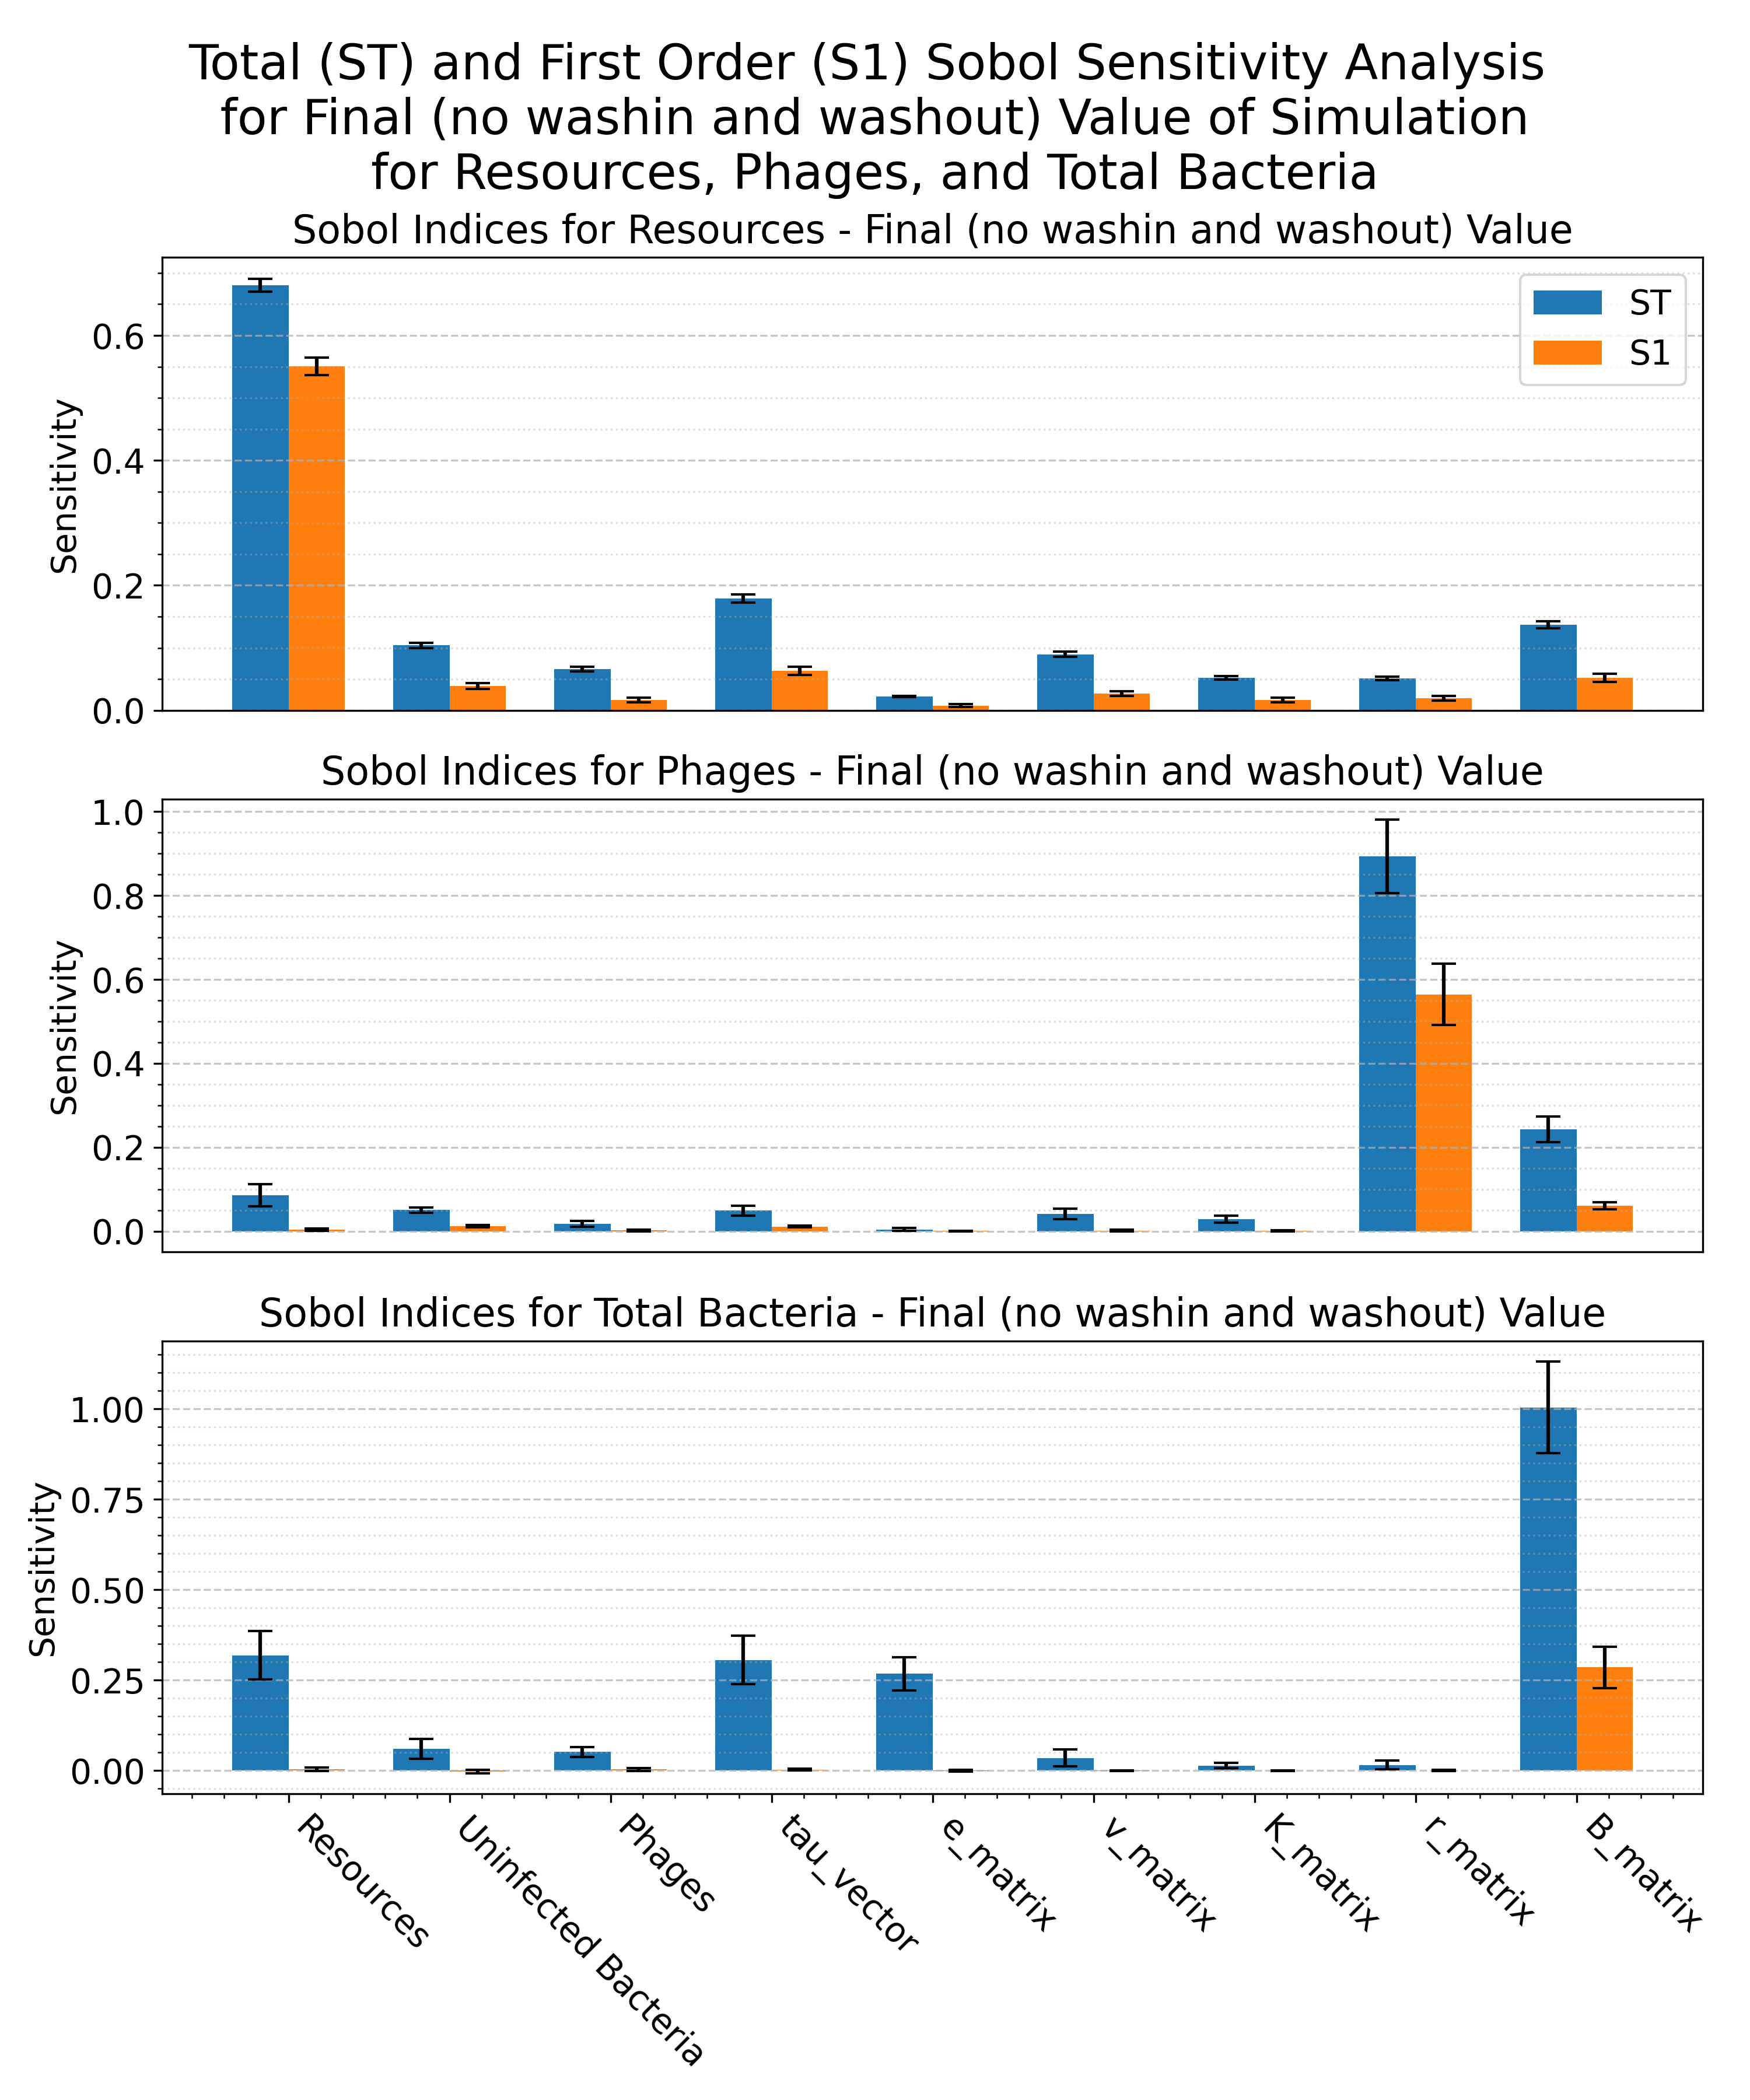
\includegraphics[width=\linewidth]{Plots/Created/SOBOL/SOBOL_analysis_1749708738_Final_(no_washin_and_washout).png}
        \caption{
            The final value, with no washin and washout. 
        }
        \label{fig:created:Sobol_final_no_wi_wo}
    \end{subfigure}
    \hfill
    \begin{subfigure}{0.32\linewidth}
        \centering
        \captionsetup{width=1\linewidth}
        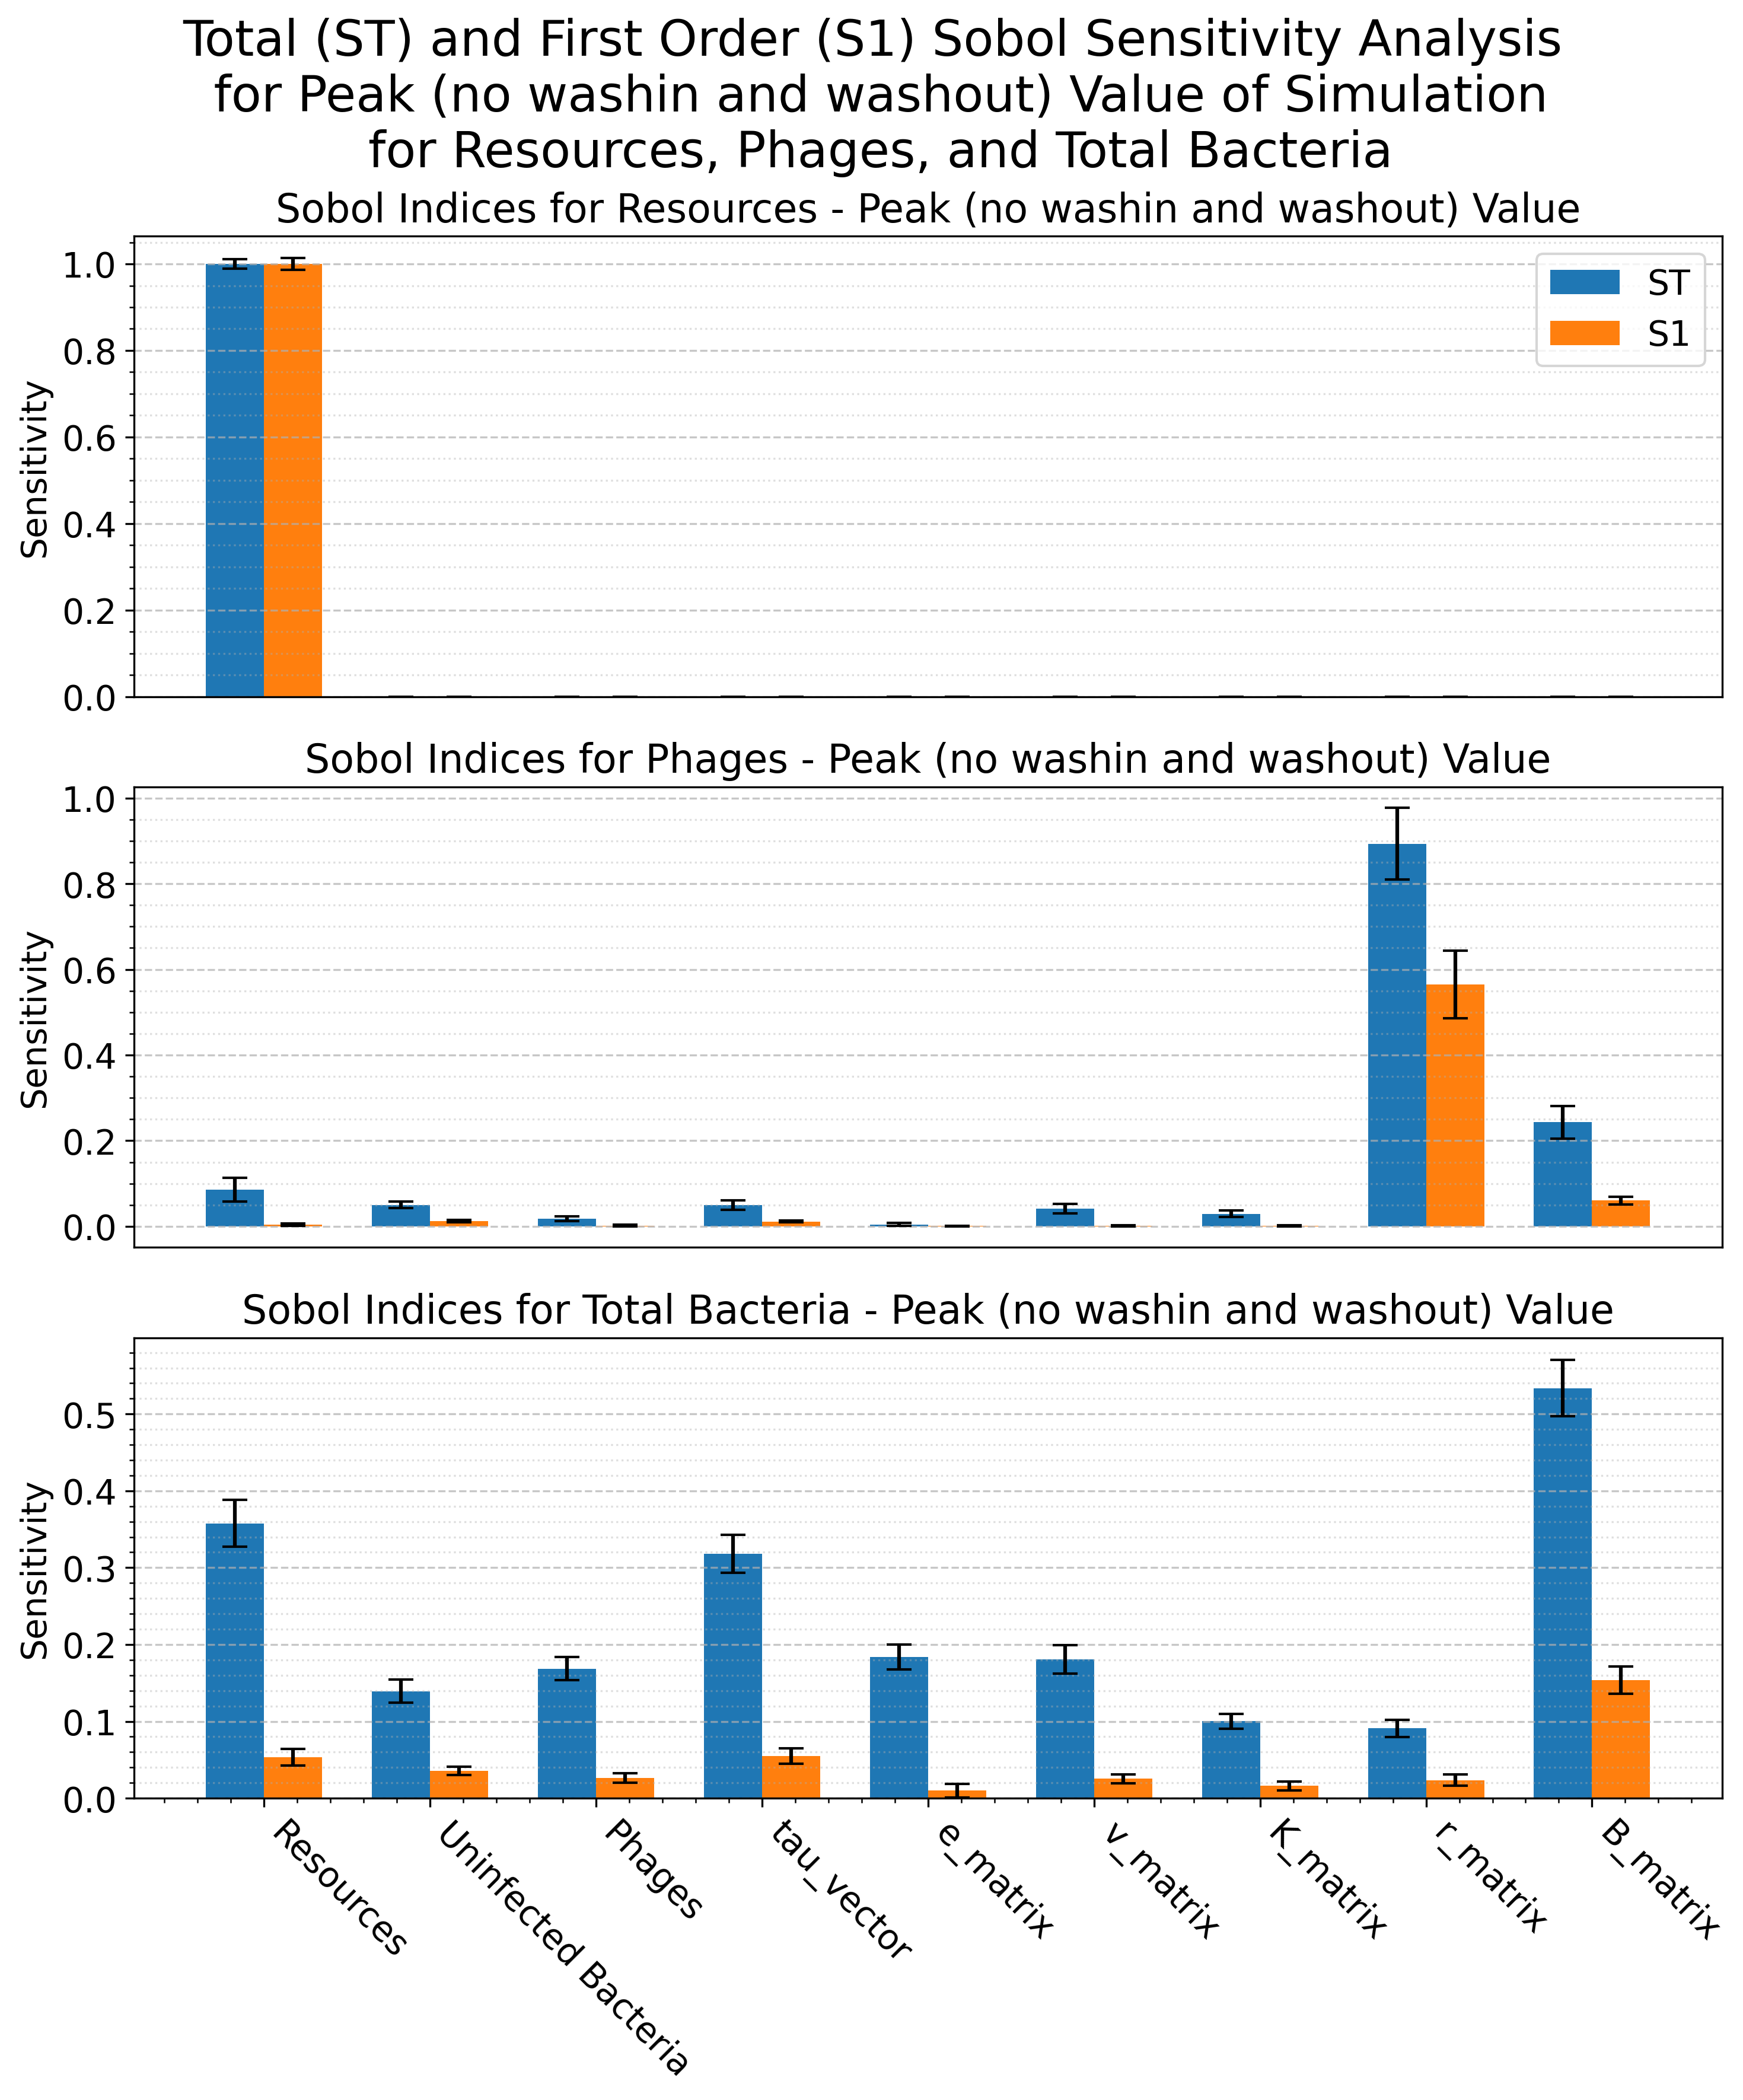
\includegraphics[width=\linewidth]{Plots/Created/SOBOL/SOBOL_analysis_1749708738_Peak_(no_washin_and_washout).png}
        \caption{
            Peak population value, no washin, and washout. 
        }
        \label{fig:created:Sobol_peak_no_wi_wo}
    \end{subfigure}
    \hfill
    \begin{subfigure}{0.32\linewidth}
        \centering
        \captionsetup{width=1\linewidth}
        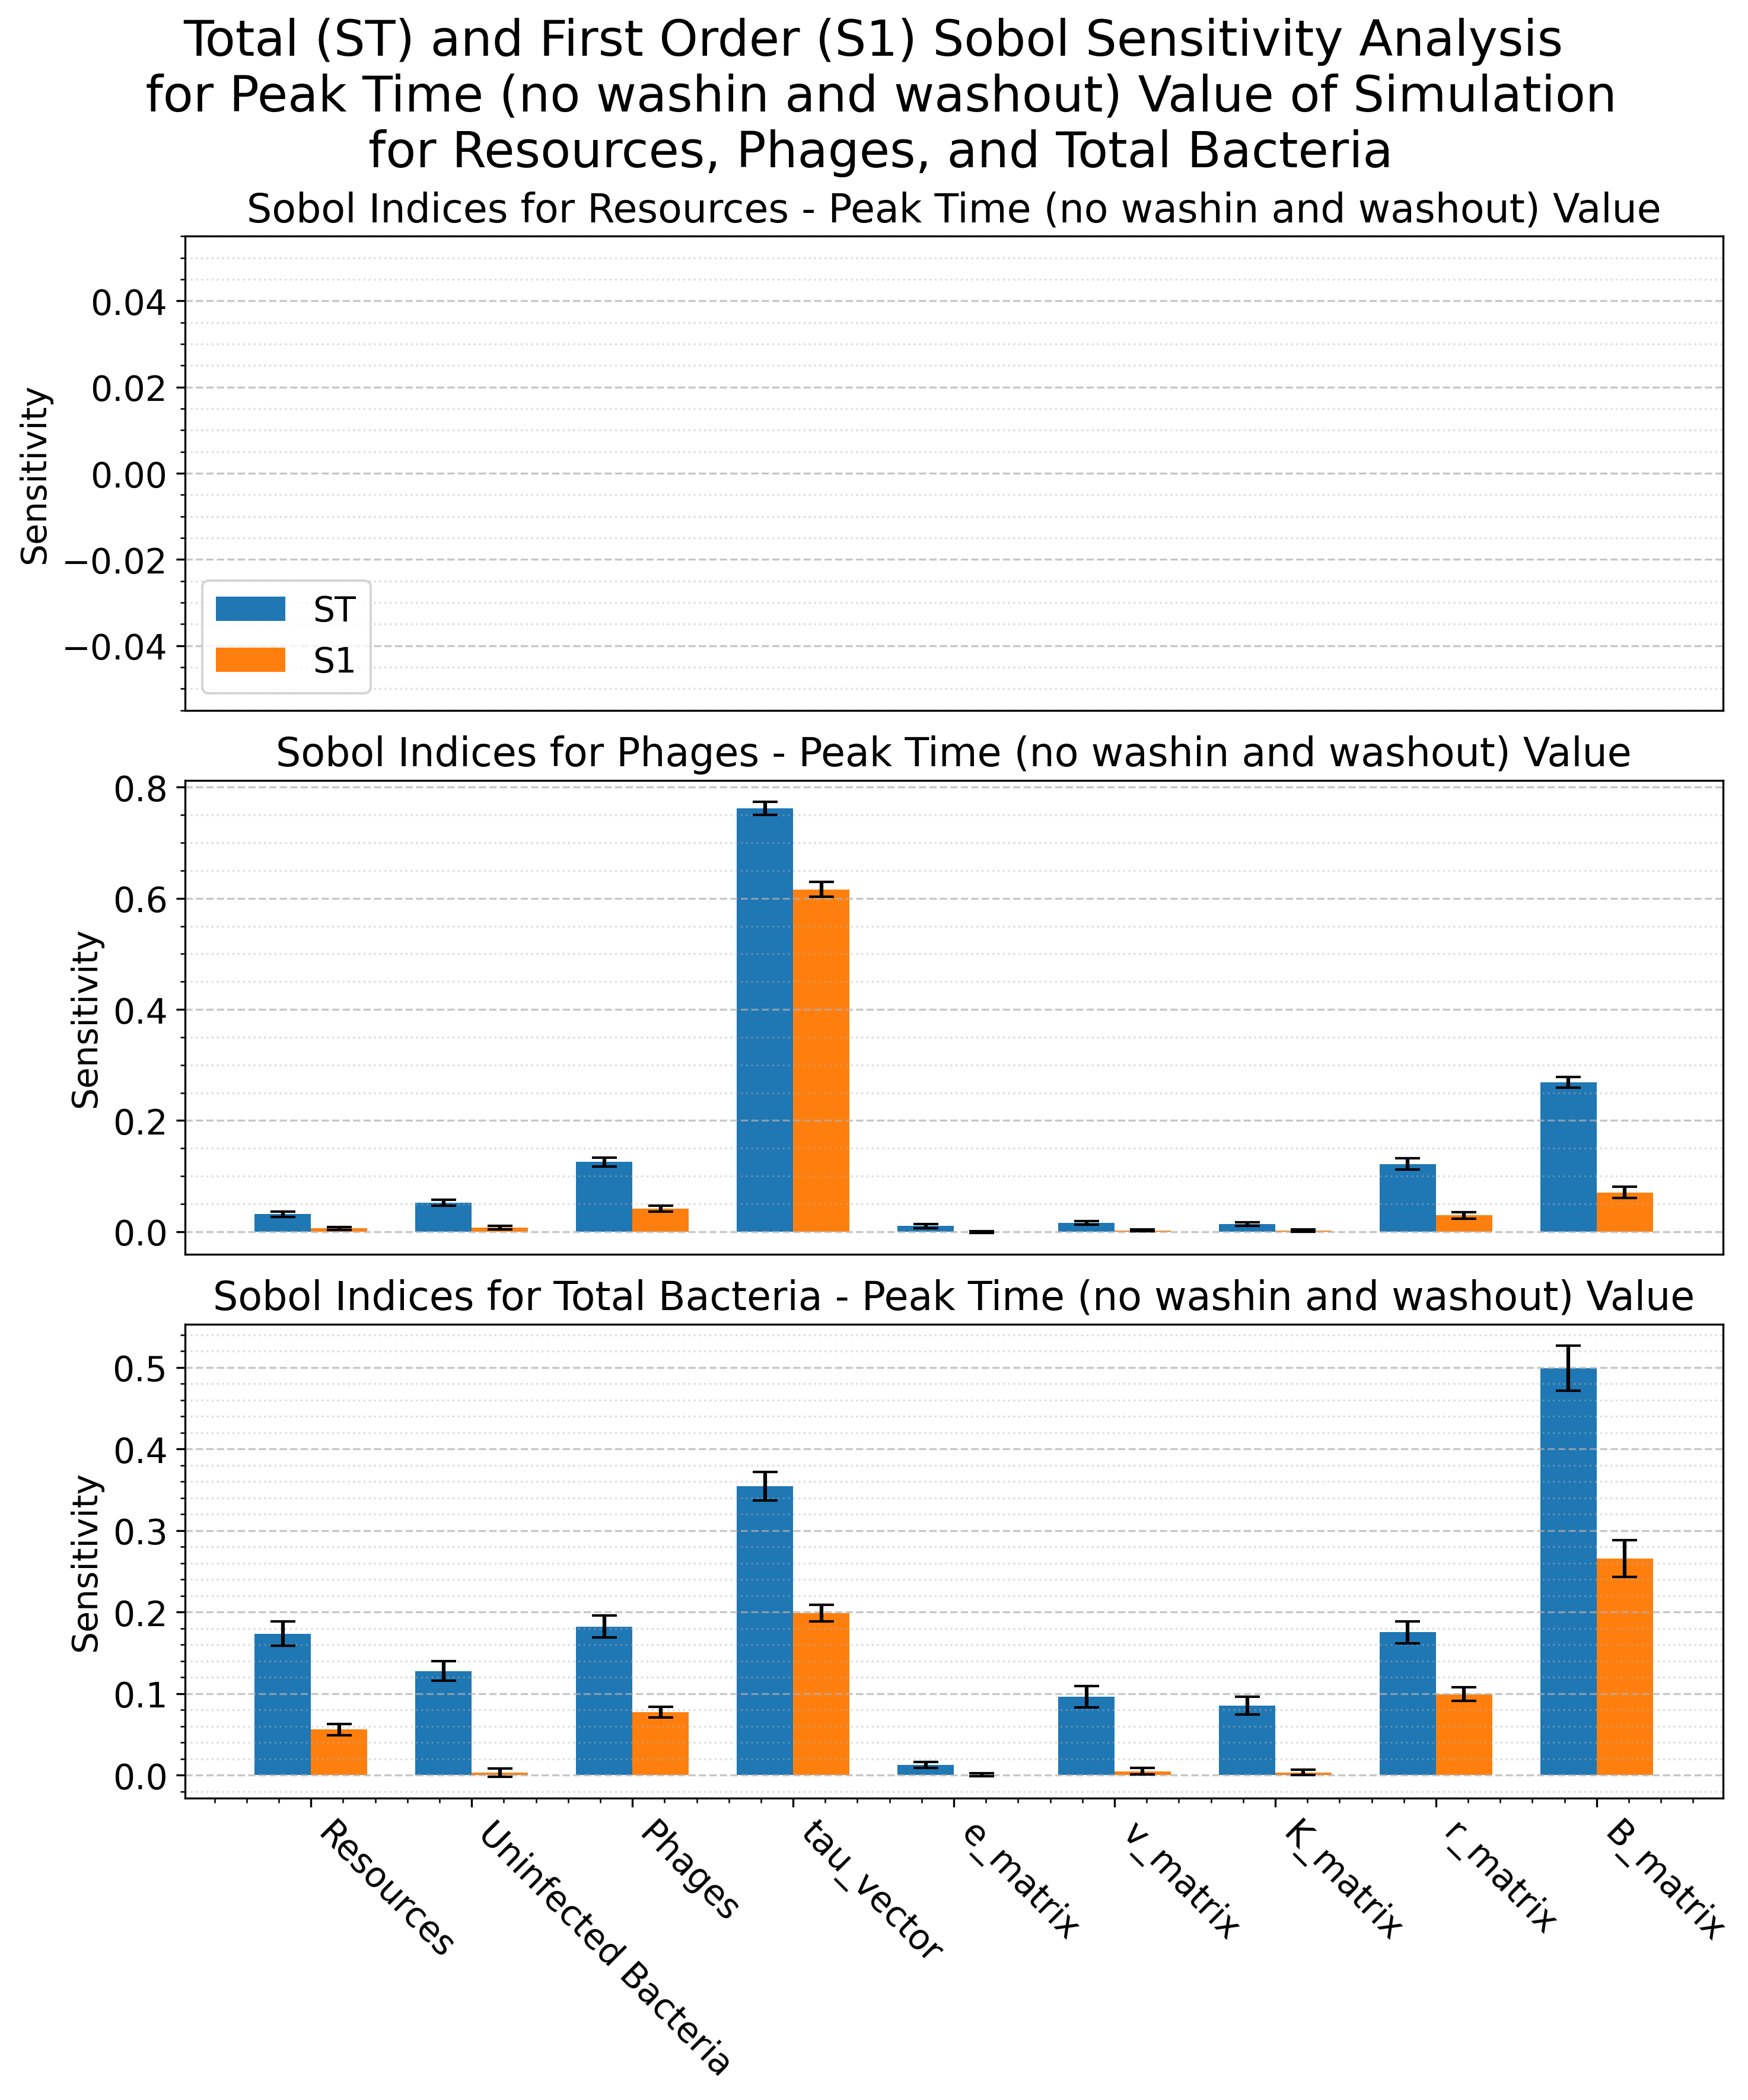
\includegraphics[width=\linewidth]{Plots/Created/SOBOL/SOBOL_analysis_1749708738_Peak_Time_(no_washin_and_washout).png}
        \caption{
            Time of peak value, no washin, and washout. 
        }
        \label{fig:created:Sobol_peak_time_no_wi_wo}
    \end{subfigure}
    \caption{
        Sobol analyses for the final, peak, and time of peak value without a washin and washout rate.
        The input value ranges to test each parameter used for this Sobol test can be found in \Cref{tab:appendixE:Sobol_analysis_values}, except that washin and washout is set to 0. 
    }
    \label{fig:created:Sobol_no_wi_wo}
\end{figure}

\section{Graph Behavior with IVA}
\label{sec:results:graph_behavior}
Understanding how a change in parameter values across a wide range of values affects the curve is essential for comprehending how the model operates across a variety of values. 
The sections below provide both quantitative and qualitative elaborations on how changes in parameter values across multiple values alter the shape of the population curves. 
Only the most critical parameters identified in the Sobol section, along with the initial resource, uninfected bacteria, and phage value, will be analyzed. 
Initially, the resources, uninfected bacteria, phage, $\tau$, $r$, and $\beta$ will be analyzed. 
The default parameter values can be found in \Cref{tab:appendixE:a_good_curve} but are given in the text as well. 
The sections below use an IVA run to analyze the change in behavior across a wide range of values. 
Each figure from which the conclusions are made can be found in \Cref{sec:apendixF:graph_behavior_with_IVA}. 
$\omega^i$ and $\omega^o$ are not included despite having a considerable impact as seen in \Cref{sec:AppendixF:sobol_analysis_with_washin_and_washout} because $\omega^i$ and $\omega^o$ are not a part of the original Golding model. 
Some of the results are unrealistic and do not accurately replicate real-life growth curves. 

\subsection{Initial Resource $R$}
The initial resource $R$ concentration values were tested across a range from 1 resource to 500 resources, with a default value of 200 resources. 
The IVA results can be found at \Cref{fig:created:IVA_IVAtable_resource}. 
All resource values are depleted at around the same time, within 1 time unit of each other. 
As the resource concentration increases, the time it takes for the uninfected bacteria to reach its peak population increases from 0.5-time units to 4.12-time units. 
The infected bacteria face the opposite, whereas the resource concentration increases, and the time to peak decreases from 9.5-time units to 4.9-time units. 
The same behavior is exhibited for the phages, except that the time duration changes from 14-time units to 6.3-time units. 
The phage population showed a significant variation in maximum population, ranging from a maximum of 464 phages to 17,200 phages, a 37-fold difference. 
The maximum bacterial population sum varied from 55 to 3106 total bacteria, representing a 56.5-fold difference. 

\subsection{Initial Uninfected Bacteria $U$}
The initial uninfected bacteria $U$ population values were tested across a range of 1 to 100 uninfected bacteria, with a default value of 20 uninfected bacteria. 
The IVA results can be found at \Cref{fig:created:IVA_IVAtable_uninfected_bacteria}. 
As the initial uninfected bacterial population increases, resources are consumed at a faster rate, and the bacterial populations grow more rapidly and peak earlier. The phages were able to grow faster. 
The phages peaked at 5.7-time units for 100 initial uninfected bacteria, whereas for small initial uninfected populations, the phages peaked at 10.3-time units. 
Varying the number of uninfected bacteria had little influence on the maximum value reached. There is a difference of 600 phages between the phages that started with 1 uninfected and 100 uninfected bacteria. 
The difference in total bacteria peak values is 173. 
Changing the uninfected bacteria had little influence on the peak values but had a significant impact on the time at which the peak value occurred. 

\subsection{Initial Phage $P$}
The initial phage $P$ population values were tested across a range from 1 phage to 50 phages, with a default value of 10 phages. 
The IVA results can be found at \Cref{fig:created:IVA_IVAtable_phages}. 
The differing phage values had almost no influence on resource consumption and a limited impact on the peak value and time to peak value for both the bacteria and phages. 
The difference between the peak and time of peak values is minor. 
The final phage population at $t=15$ was 9,436, for an initial phage value of 50. In contrast, for an initial phage value of 1, the final phage value reached 10,676. 
The time of peak difference is just 1.44-time units. 
As the phage value increases, the time required for the uninfected, infected, and phage populations to reach their peak values decreases. 

\subsection{Latency Period $\tau$}
The latency period $\tau$ parameter values were tested across a range from 0.5 to 3.5, with a default parameter value of 0.7. 
The IVA results can be found at \Cref{fig:created:IVA_IVAtable_tau}. 
$\tau$ does not influence how fast the resources are being consumed. 
However, as $\tau$ increased, the time for the infected bacteria population to peak went from 4.43 to 11.21-time units, and the time it took for the phages to peak went from 5.49 to 14.70-time units, 2.53 times, and 2.68-times increase in time length. 
Smaller $\tau$ values resulted in larger final phage populations and smaller total bacteria populations. 
The peak value and time of peak value for varying $\tau$ values show little difference for the bacteria sum, ranging from a peak of 1,444 to 1,702 total bacteria and a time of the peak of 3.74 to 3.82-time units, a difference of 0.08-time units. 
As $\tau$ increases, the infection process will take longer, and it will take longer for the bacteria to die. 
Dying later means the phage’s population experiences a delay in growth, taking longer to reach its peak population value. 
Meanwhile, more bacteria can grow and consume resources. 
The bacteria will take longer to peak as there is less initial pressure from the phages. 

\subsection{Adsorption Rate $r$}
The adsorption rate $r$ parameter values were tested across a range from 0.001 to 0.2, with a default parameter value of 0.001. 
The IVA results can be found at \Cref{fig:created:IVA_IVAtable_r}. 
For small $r$ values, all resources are consumed by $t=5$, while for large $r$ values, only 13.12 resources were consumed as not enough bacteria were created throughout the simulation to consume all the resources. 
As $r$ increases, the time to reach the max value decreases for the uninfected and infected bacteria and phages. The delay in phage value decreased from 6.32 to 2.35-time units, and the total bacteria decreased from 3.81 to 0.59-time units. 
However, for large $r$ values, there was little growth of phage and bacteria. 
For large $r=0.2$ values, the maximum number of phages and bacteria was 154 and 79, while for small $r=0.001$ values, the maximum number of phages and total bacteria was 10,464 and 1,588, respectively. 
As $r$ increases, the probability of a successful infection increases, thereby enhancing the adsorption rate of phages and causing them to grow and peak earlier. 
This higher adsorption rate causes the bacteria to become infected more quickly, resulting in their faster death. 
Lower $r$ values allow the bacteria to grow for an extended period, providing more bacteria for the phages to infect, which in turn leads to higher final phage populations.

\subsection{Burst Size $\beta$}
The burst size $\beta$ parameter values were tested across a range from 1 to 100, with a default parameter value of 10. 
The IVA results can be found at \Cref{fig:created:IVA_IVAtable_beta}. 
For large $\beta$ values, not every resource was consumed, similar to large $r$ values, where for $\beta=100$, 89 resources were consumed. 
As $\beta$ increases, the time to peak for the infected bacteria and phages temporarily increases before decreasing. 
For the uninfected bacteria, the time to peak (does not change for $\beta=1$ to $\beta=10$) takes 3.8-time units, but for larger $\beta$ values, the time to peak decreases to a minimum of 1.94-time units. 
There was a significant difference in phage population values, ranging from 4.54 final phages to 42,570 phages, representing a 9,376-fold increase in phage value. 
As $\beta$ increases in value, more phages are being created upon lysis, which infects the bacteria. 
For $\beta$ less than 10, bacterial growth is restricted by latency, which determines how fast a bacterium can complete the infection process. At the same time, for $\beta$ greater than 10, the system transitions to an adsorption-limited regime, where phages cannot adsorb to the bacteria quickly enough, allowing the bacteria to grow more rapidly and reach a peak earlier. 
As phage production increases, more bacteria become infected, causing the bacterial population to decline earlier and leading to reduced bacterial reproduction. 
With fewer bacteria present, resource consumption also decreases.

\section{Initial Value Analysis Results}
\label{sec:results:initial_value_analysis}
\Cref{fig:created:initial_value_analysis_UB_50_500_a_good_plot_2} and \Cref{fig:created:initial_value_analysis_UB_50_500_a_good_plot} illustrate how varying the initial uninfected bacteria population from 1 to 500 (using 100 different starting values) affects the dynamics and time of peak population of phage and total bacteria populations using the 95\% rule. 

\Cref{fig:created:initial_value_analysis_UB_50_500_a_good_plot_2} perfectly replicates Figure 1 of \citet{mullaExtremeDiversityPhage2024} (\Cref{fig:sourced:Mulla}). 
As the initial bacteria population increases, the time to reach the phage and bacteria sum peak decreases, following $y = -0.8648\cdot ln(x) + 9.7911$ and $y = -1.0056\cdot ln(x)+7.7626$, with $R^2=0.9800, 0.9988$ respectively. 

\Cref{fig:created:initial_value_analysis_UB_50_500_a_good_plot} on the other hand shows different behavior. 
As the initial bacteria population decreases from 500 to 100, \Cref{fig:created:initial_value_analysis_UB_50_500_a_good_plot_2} exhibits the same behavior. 
There is a change in behavior at 100 and less initial uninfected bacteria. 
Instead of following the predicted line like in \Cref{fig:created:initial_value_analysis_UB_50_500_a_good_plot_2}, the curve for the phages decreases non-monotonically.
The bacteria plateau before starting to increase again. 
The fitted linear regression curves follow $y = -0.1292\cdot ln(x) + 10.1462$ and $y = -0.6234\cdot ln(x)+6.9602$, with $R^2=0.5406, 0.9206$ respectively. 

The slope tells us how well the uninfected bacteria influence the time of peak value. 
The larger (positive or negative) the slope is, the greater the impact the uninfected bacteria have on the time of peak value. 
The closer the $R^2$ value is to 1, the greater the proportion of the variance in the time to peak value is explained by the uninfected bacteria. 
The linear regression curve can not explain the change in limiting regions. 
For the first curve, the uninfected bacteria had a small influence on the time of peak value. 
In contrast, for the second curve, changing the number of uninfected bacteria had a more significant impact on the time of peak and is considerably more important in explaining the time of peak value. 

\begin{figure}
    \centering
    \begin{subfigure}{1\linewidth}
        \centering
        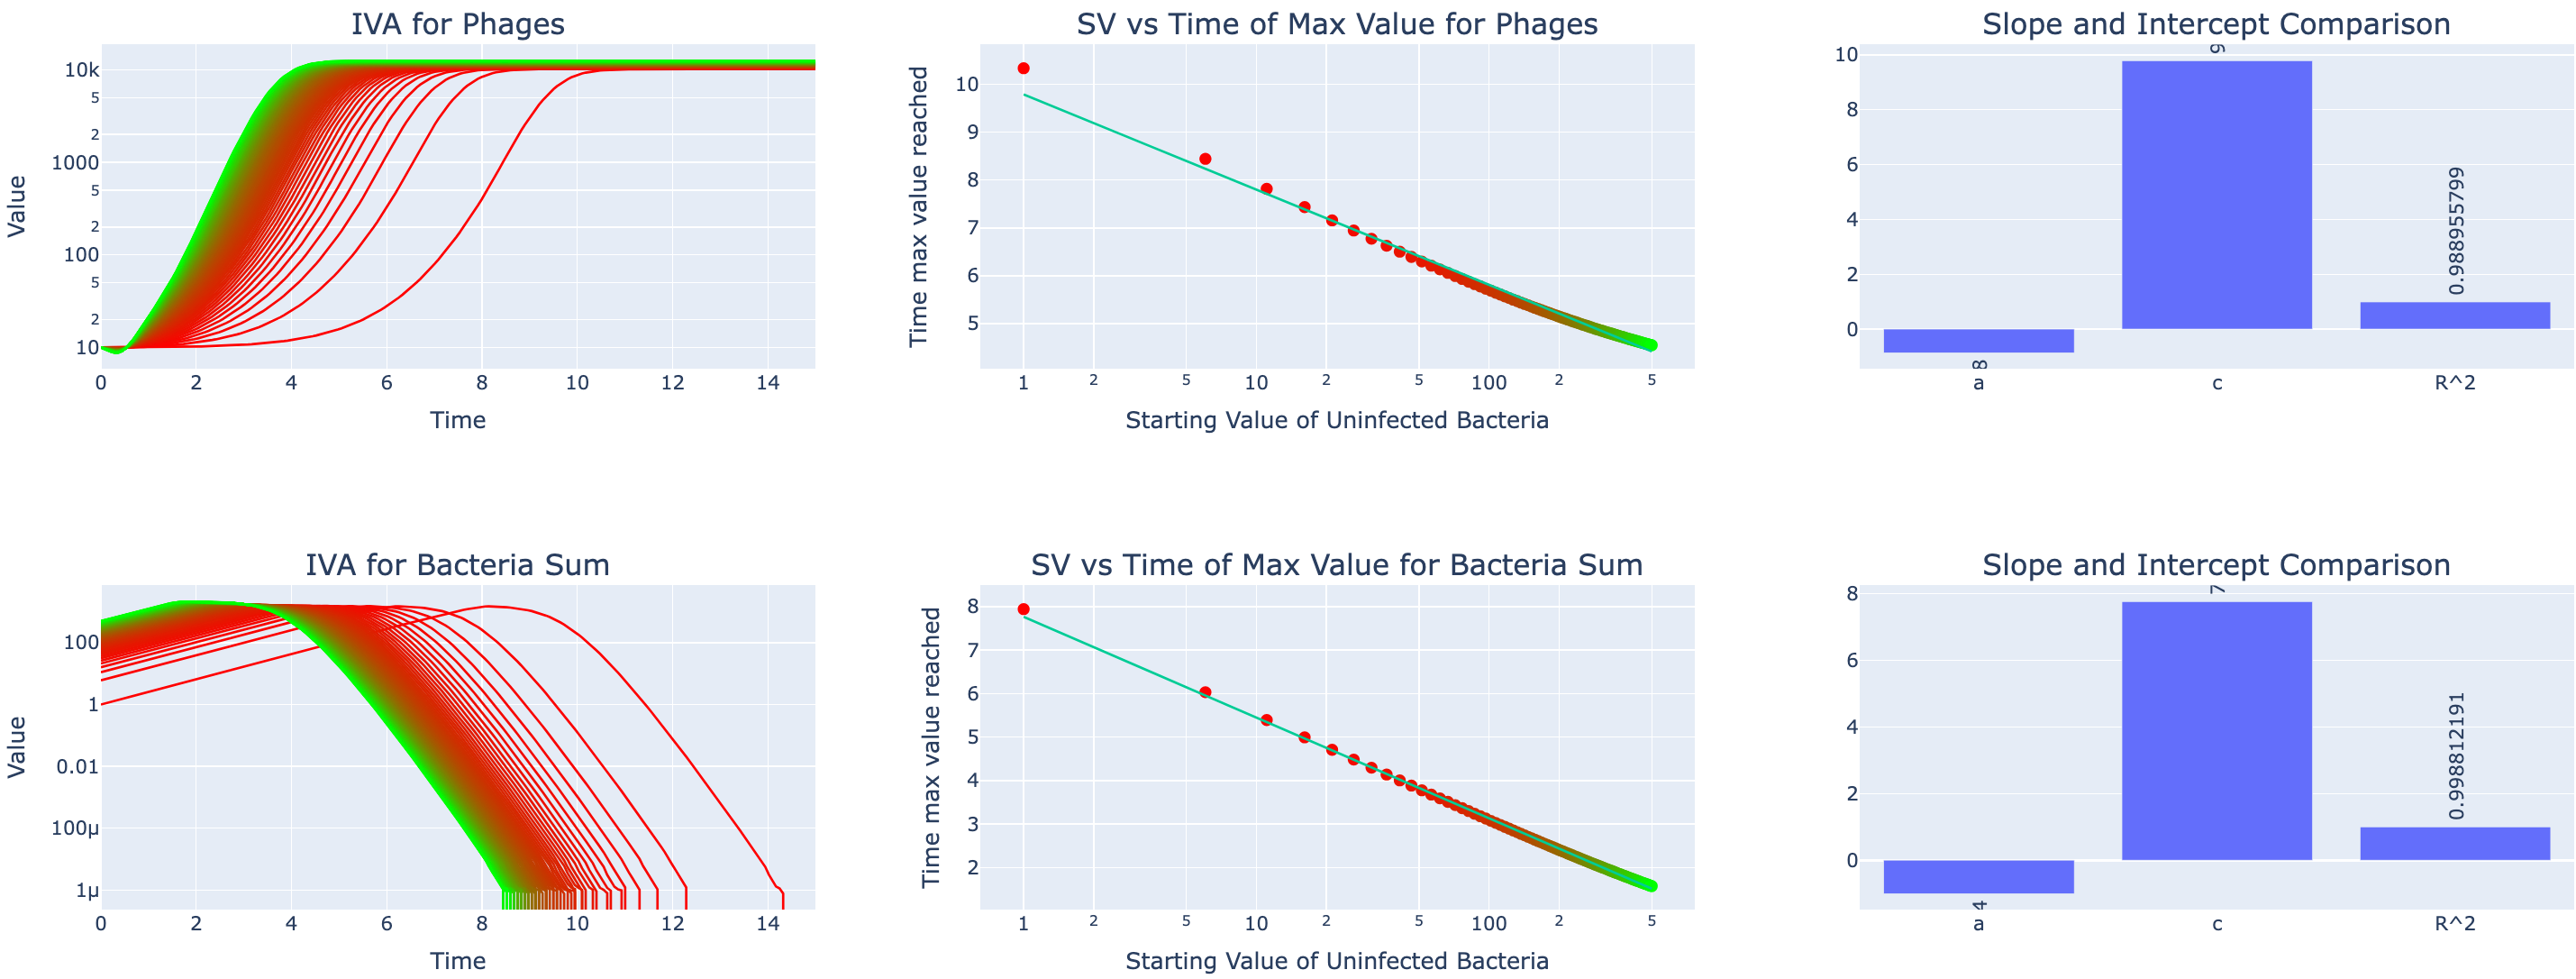
\includegraphics[width=\linewidth]{Plots/Created/IVA/initial_value_analysis_UB_50_500_a_good_plot_2.png}
        \caption{
            IVA for \Cref{tab:appendixE:a_good_curve_2}. 
            Replicates Figure 1 of \citet{mullaExtremeDiversityPhage2024}. 
            The system is adsorption limited \cite{mullaExtremeDiversityPhage2024}. 
        }
        \label{fig:created:initial_value_analysis_UB_50_500_a_good_plot_2}
    \end{subfigure}
    \hfill
    \begin{subfigure}{1\linewidth}
        \centering
        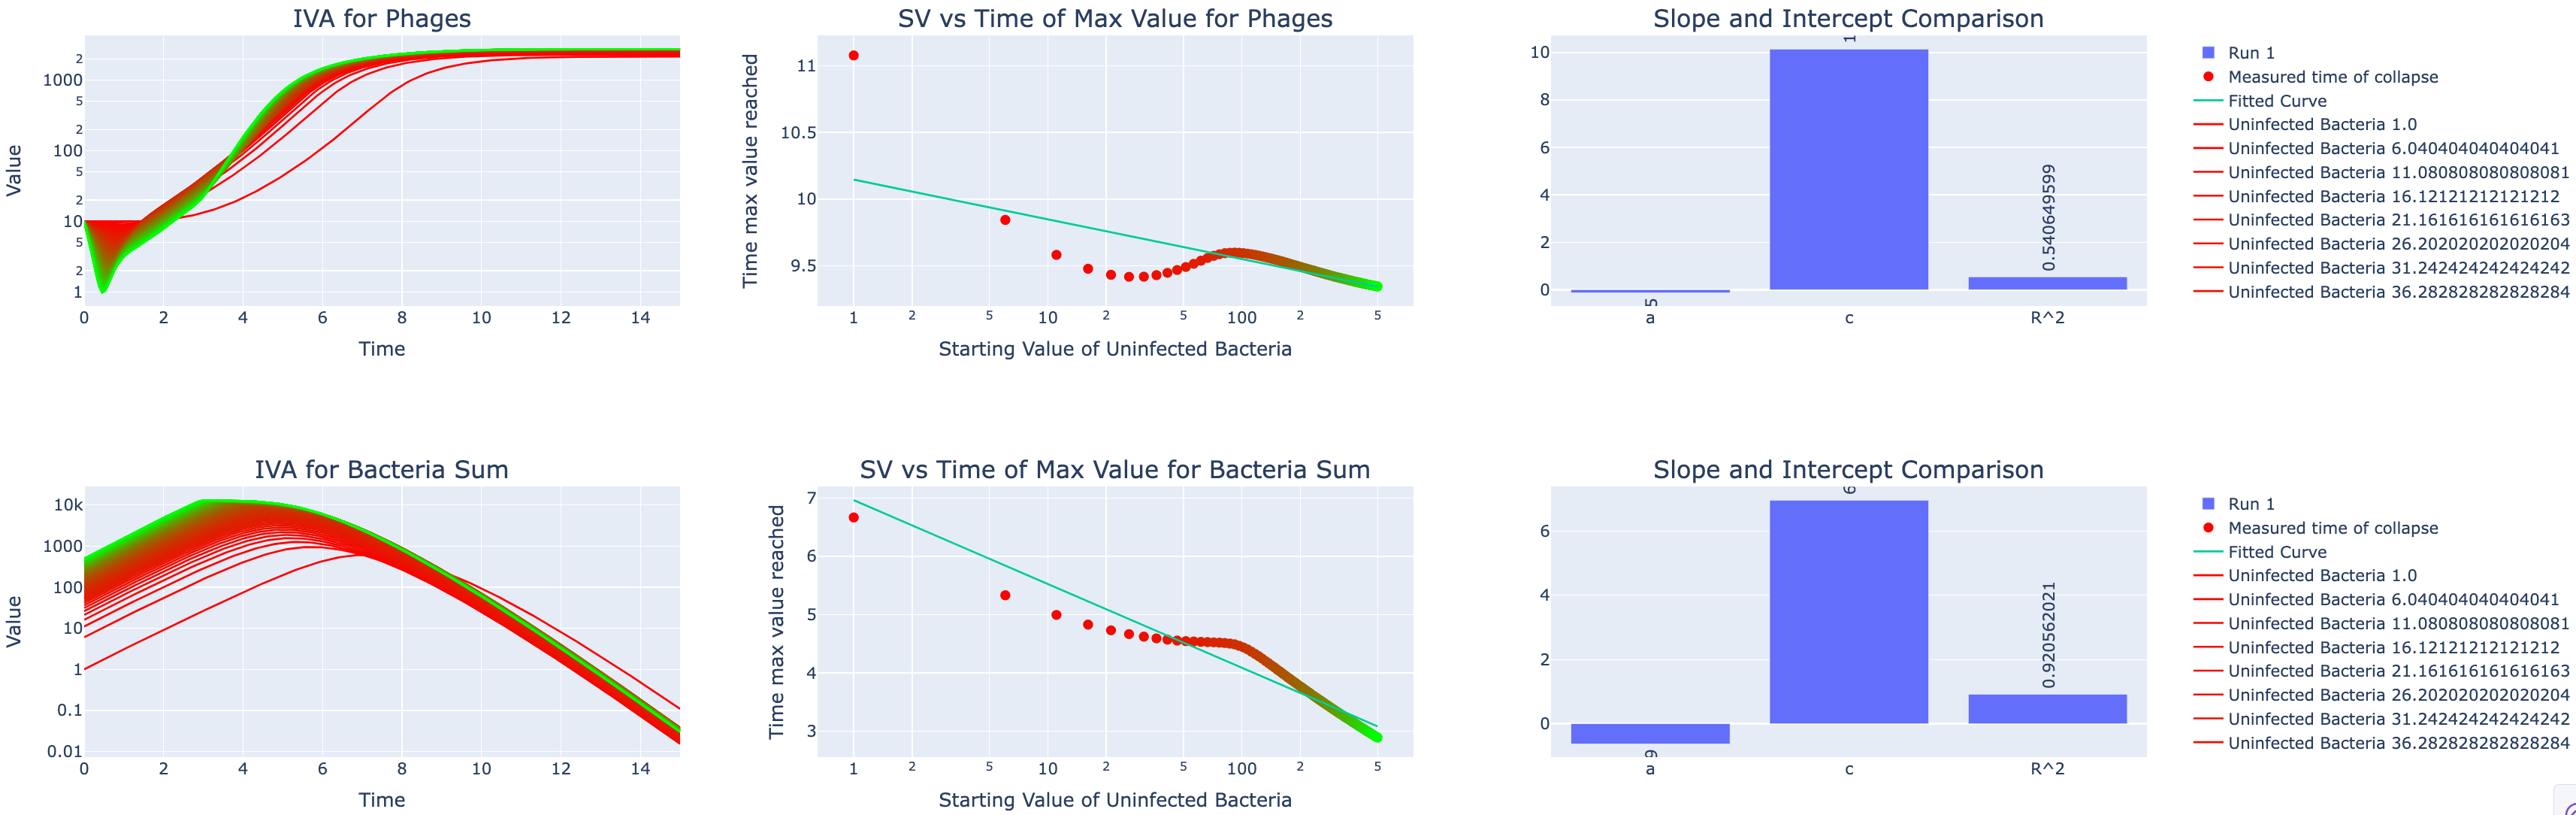
\includegraphics[width=\linewidth]{Plots/Created/IVA/initial_value_analysis_UB_50_500_a_good_plot.png}
        \caption{
            IVA for \Cref{tab:appendixE:a_good_curve}. 
            For initial uninfected bacteria of less than 100, the phage-bacteria interaction is burst-limited, whereas for initial uninfected bacteria of more than 100, the phage-bacteria interaction is adsorption-limited. 
        }
        \label{fig:created:initial_value_analysis_UB_50_500_a_good_plot}
    \end{subfigure}
    \caption{
        Varying the initial uninfected bacteria concentration, from 50 to 500, with 30 unique values tested. 
        Varying the default parameter values can have a significant impact on how changing the initial bacterial concentration affects the system’s dynamics. 
        The default values for Figures a) and b) can be found at \Cref{tab:appendixE:a_good_curve} and \Cref{tab:appendixE:a_good_curve_2}. 
    }
\end{figure}

\section{Phage Proliferation}
Understanding how phage behavior varies under different conditions is essential. 
Phages can experience chemical or biological deactivation or, if the replication process is not fast enough, be removed from the system through washout. 
It is very easy for a researcher to vary the initial resource concentration, phage, or resource concentration. 
One of the first experiments that a researcher might conduct in a lab is to investigate how changing the initial population or concentration value of phages, bacteria, and resources affects the survival of phages or bacteria and by how much. 

\subsection{Phase Portrait}
\label{sec:results:phase_portrait}
Comparing a phage, bacteria, and resource value against one another can reveal how one population evolves in relation to another over time. 
It is easier to understand how one population evolves compared to a change in another population. 
It also illustrates how initial population values can influence the evolution of populations in relation to one another. 

\Cref{fig:created:phase_portrait_resources_245-265_phages_25-26} shows a phase portrait varying the initial resource and phage concentration. 
The exact initial phage values have the same color for the line. 
For phages that start at a population above 25.98, the phage population can proliferate until the washout eventually removes the phages. 
For phage populations that start below 25.98, the washout removes the phages before they have time to infect and kill the bacteria. 
Both regions of phages exhibit consistent behavior, either going to 0 or proliferating. 
If the phage population started at precisely 25.98, if the initial resources were 260 or above, the phages died out. 
If the initial resource value was 255 or below, the phages proliferated. 

\subsection{An Initial Resource and Phage Value Analysis for Phage Proliferation}
\Cref{fig:created:phase_portrait_resources_phage} expands on the phase portrait by simulating more values and coloring the square depending on whether the phages proliferated or not. 
The initial resource values span from 1 to 500, and the initial phage values range from 25.5 to 26.5, each with 100 unique values sampled.

\Cref{fig:created:phase_portrait_resource_phage_proliferate} zooms into the range $(1-40, 24.2-25)$ for a highly detailed view of the behavior happening around initial resources of 10. 
From 1 to around 7 initial resources, fewer phages are needed to ensure proliferation. 
At 7 initial resources, there is a minimum in the phage proliferation boundary. 
From 7 initial resources and upwards, as more resources are added to the system, more phages are needed to ensure proliferation. 
Despite this, the change is tiny, a difference of about two phages. 
Considering the range of possible initial phage populations, the phage proliferation boundary is flat. 
Under these parameter values, choosing an initial phage population of 27 or higher will ensure phage proliferation. 
The higher the initial resource concentration, the more final phages will appear. 
As there are more resources, more bacteria can grow from the resources, which in turn allows more phages to grow. 

When washout is higher, the system exhibits behavior similar to that shown in \Cref{fig:created:phase_portrait_resources_phage}, but it requires more phages to achieve proliferation. 
Increasing $K$ shifts the minimum point of the proliferation boundary to the right.
In both cases, the phage proliferation boundary is still relatively flat.  

\begin{figure}[]
    \centering
    \begin{subfigure}{0.49\linewidth}
        \centering
        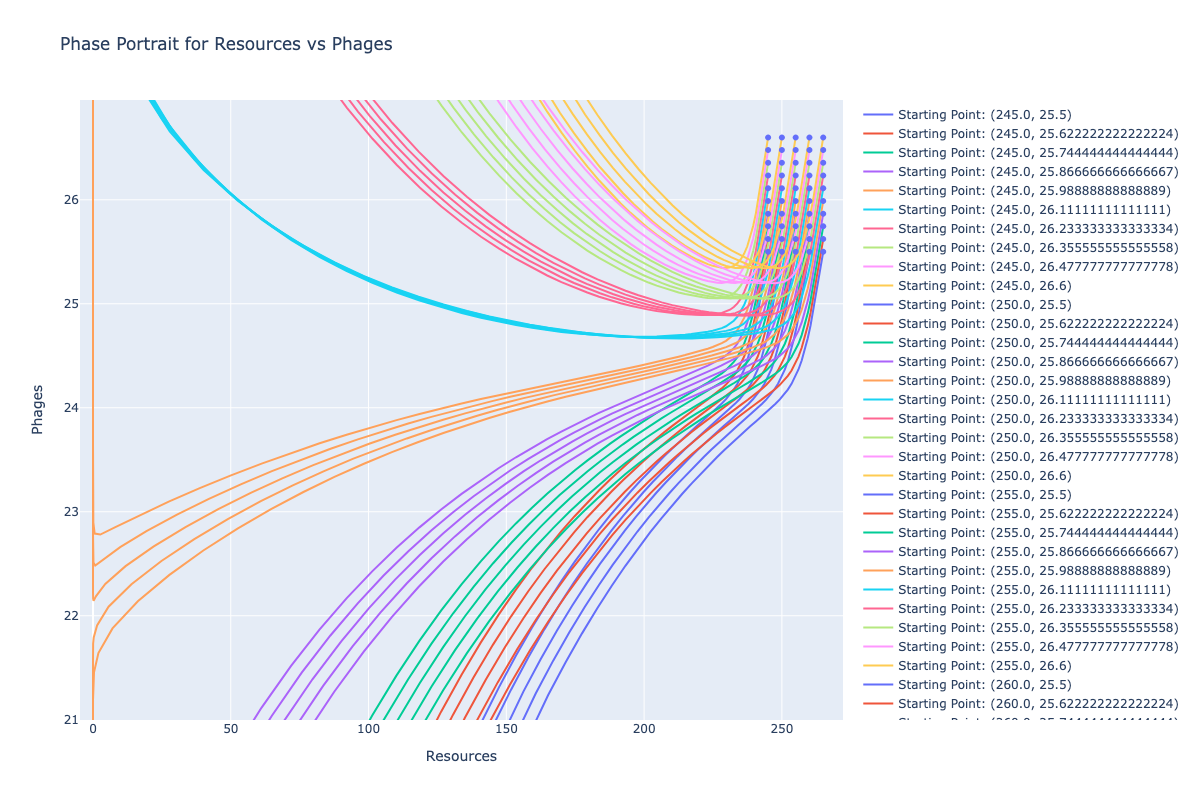
\includegraphics[width=1\textwidth]{Plots/Created/PP/phase_portrait_resources_245-265_phages_25-26.png}
        \caption{
            The zoomed-in plot of a phase portrait with varying resource and phage population from 245-265 and 25.5-26.5, respectively. 
            Each row has its own line color. 
            Diverging behavior is observed for the orange lines (when $P = 25.98$). 
        }
        \label{fig:created:phase_portrait_resources_245-265_phages_25-26}
    \end{subfigure}
    \hfill
    \begin{subfigure}{0.49\linewidth}
        \centering
        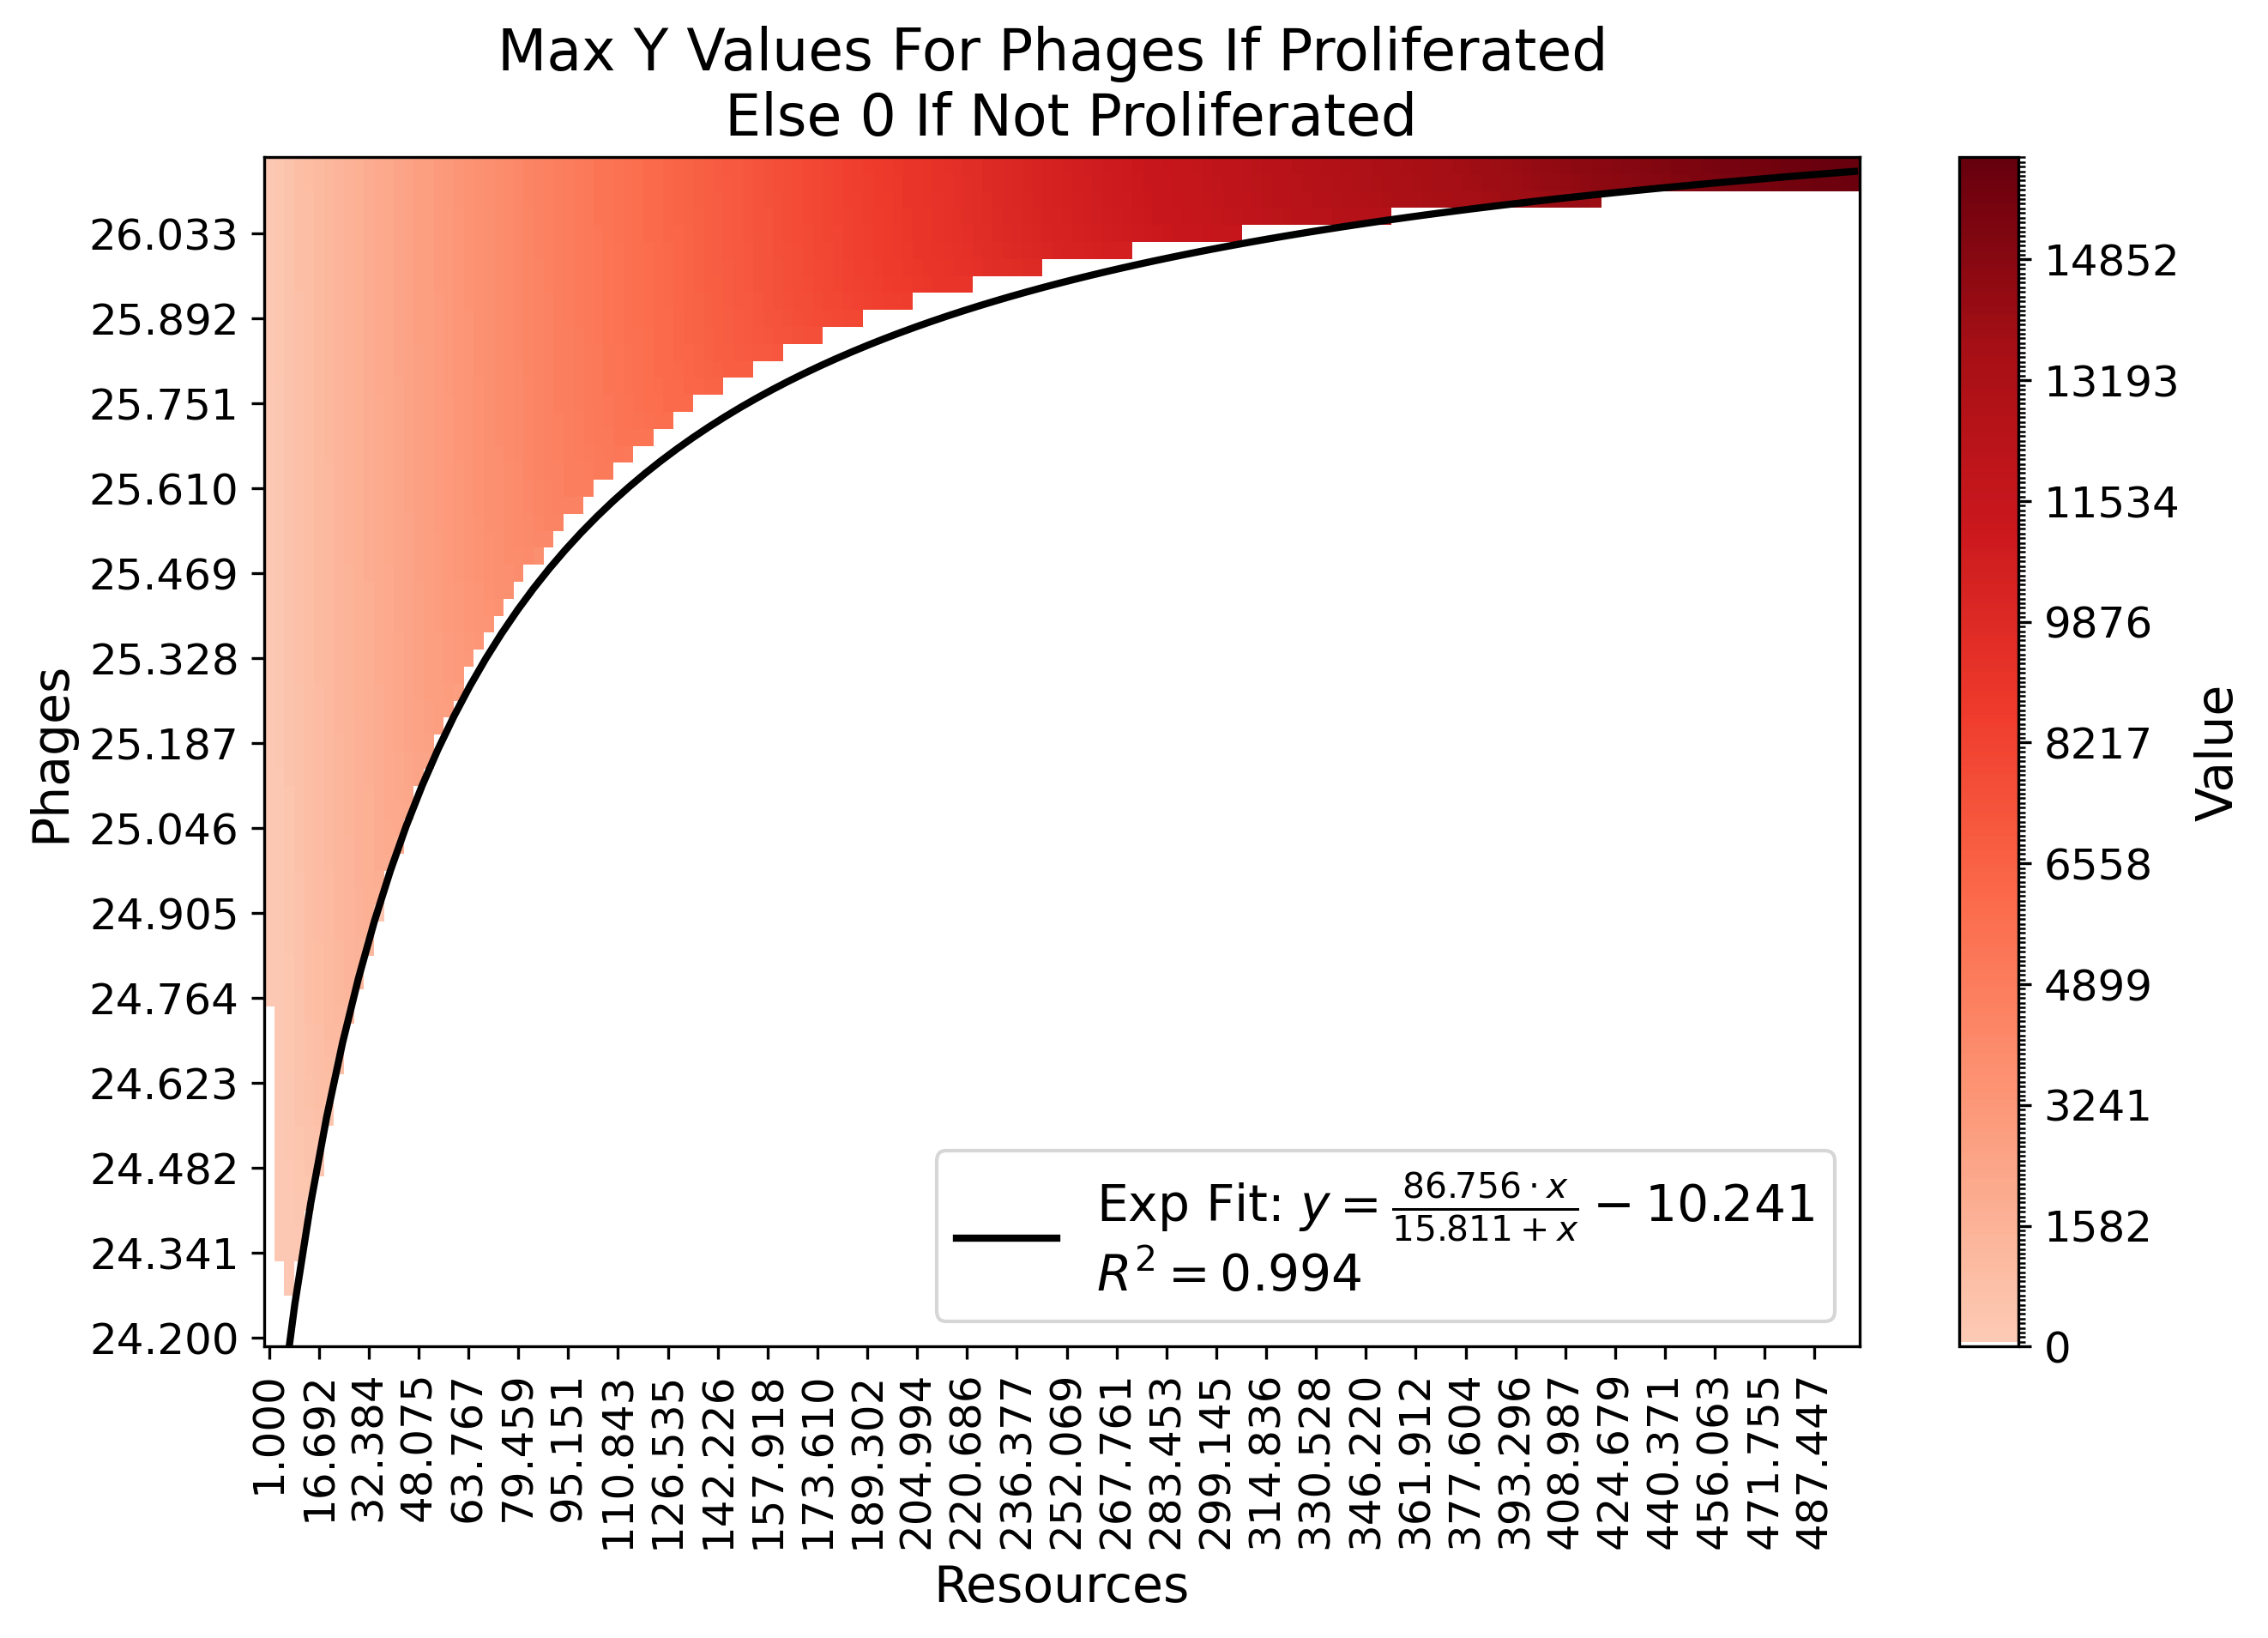
\includegraphics[width=\linewidth]{Plots/Created/PP/phase_portrait_resources_phage.png}
        \caption{
            Phage population proliferation as a function of initial resource and phage concentrations. 
            Although the color appears uniform along the vertical axis, each cell has a slightly different value. 
            The phage-resource proliferation boundary follows a fitted Monod equation.
        }
        \label{fig:created:phase_portrait_resources_phage}
    \end{subfigure}
    \hfill
    \begin{subfigure}{0.49\linewidth}
        \centering
        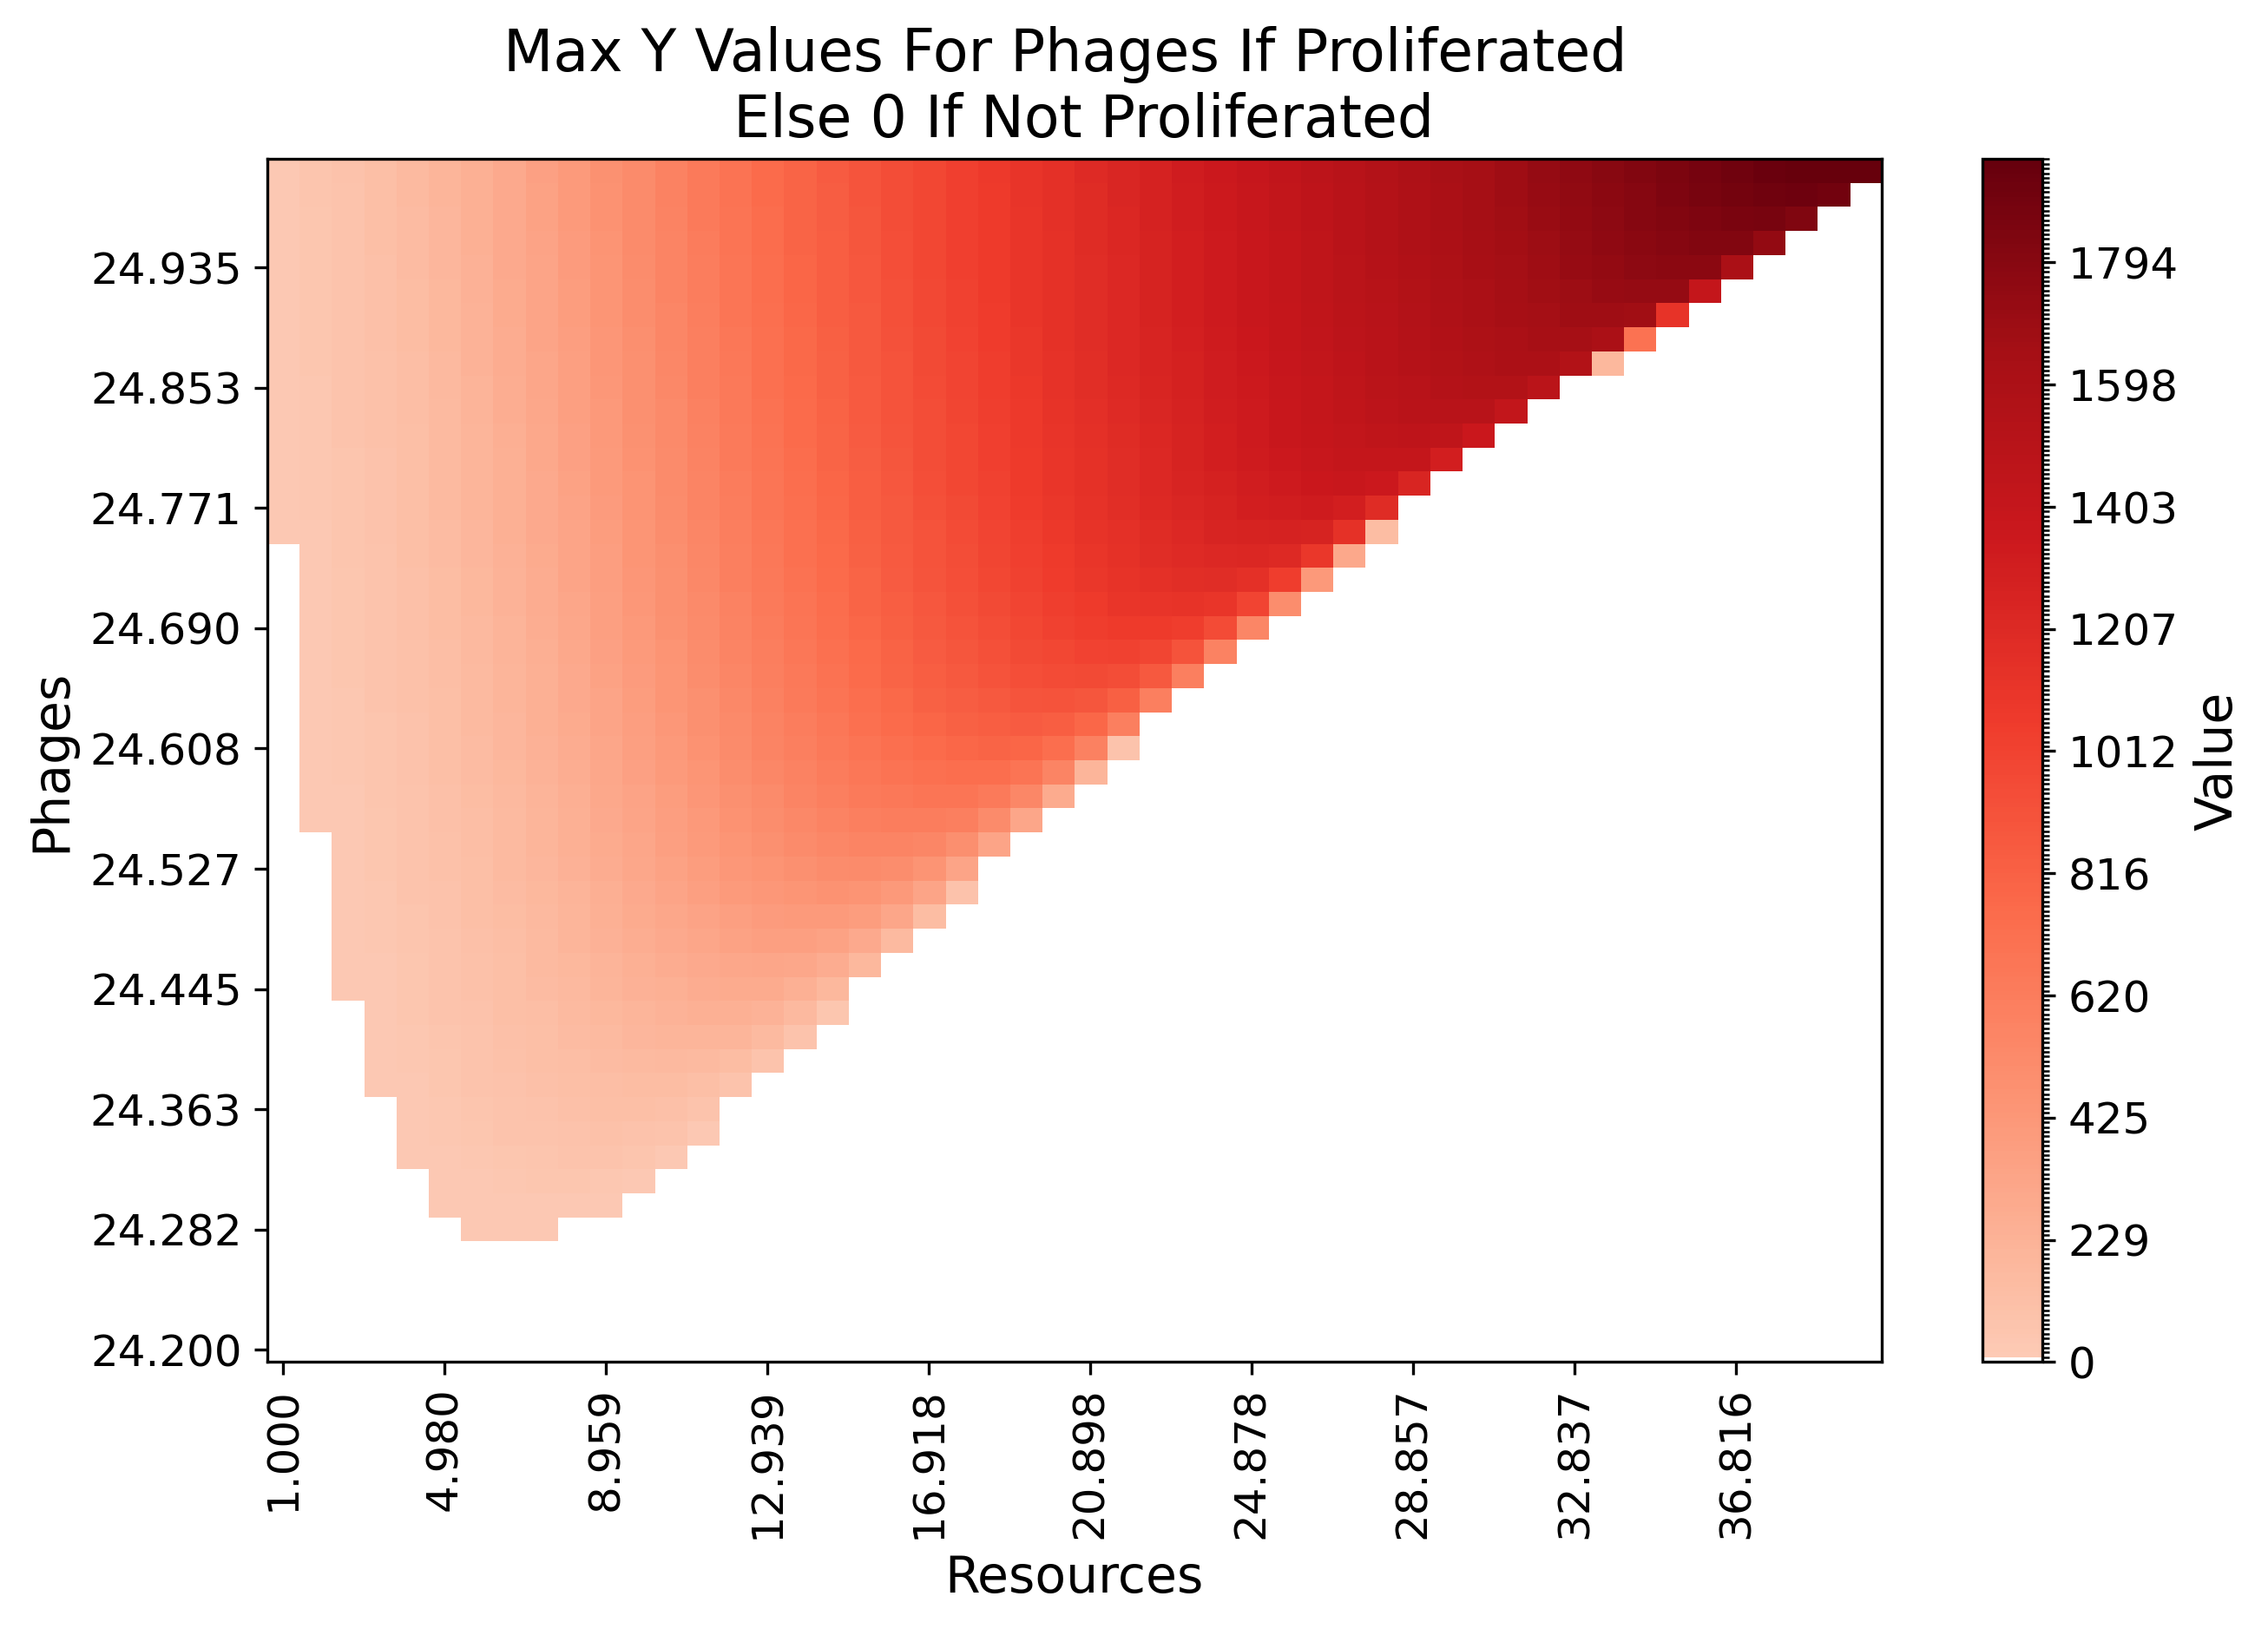
\includegraphics[width=\linewidth]{Plots/Created/PP/phase_portrait_resources_phage_2.png}
        \caption{
            Zoomed in to analyze the regime of behavior change near $R=10$. 
        }
        \label{fig:created:phase_portrait_resources_phage_2}
    \end{subfigure}
    \caption{
        Varying initial resources and initial phages and the resulting proliferation and fitted proliferation curve. 
        The box is colored red if the phages proliferated for that condition and white if the phages died out. 
        Phages proliferated if they reached twice their initial population at any point in time during the simulation. 
        This simulation used the values from \Cref{tab:appendixE:a_good_curve_2} but with washout set to 0.02 instead of 0. 
    }
    \label{fig:created:phase_portrait_resource_phage_proliferate}
\end{figure}

\subsection{An Initial Resource, Phage, and Bacteria Value Analysis for Phage Proliferation}
The initial resource concentration had some, but minimal, impact on whether the initial phage concentration would affect phage proliferation. 
Within the context of the basic Golding model, the initial uninfected bacteria population is one of three parameters that a researcher can easily control, with the other two being the initial resource and initial phage. 
For low initial populations of uninfected bacteria, it will be harder for the phages to proliferate. 
There are not enough bacteria to infect before the washout will remove the phages from the system. 
The washout $\omega^o$ removes a percentage $\omega^o$ of phages, bacteria, and resources from the system at each time step. 

For large initial uninfected bacterial populations, it will be easier for the phages to proliferate, such that the washout will not immediately eliminate the phages. 
I extend the initial resource and phage population analysis by adding a third dimension: the initial uninfected bacteria population. 
The aim of adding the uninfected bacteria is to see how the initial uninfected bacteria will: 1) affect if the phage can proliferate and 2) affect the maximum population that the phages can reach. 

\Cref{fig:created:3D_phase_portrait} has three axes: the initial phage, resource, and bacteria population value. 
The initial uninfected bacteria did not have a significant impact on two aspects: 1) whether the phages would proliferate and 2) how much the phages would proliferate. 
If sliced along the bacteria axis, there is little difference in the shape of the curve. 
It was expected that as the uninfected bacterial count increased, fewer phages would be needed to ensure phage proliferation. 
However, there is no significant change in whether the phages proliferated at all and by how much. 

This finding suggests that, under a washout situation, ensuring there are enough phages is the most critical factor among the initial phage, bacteria, and resource values to prevent the phages from being washed out. 
Conversely, changing the initial resource concentration determines the number of created phages. 

\begin{figure}[ht!]
    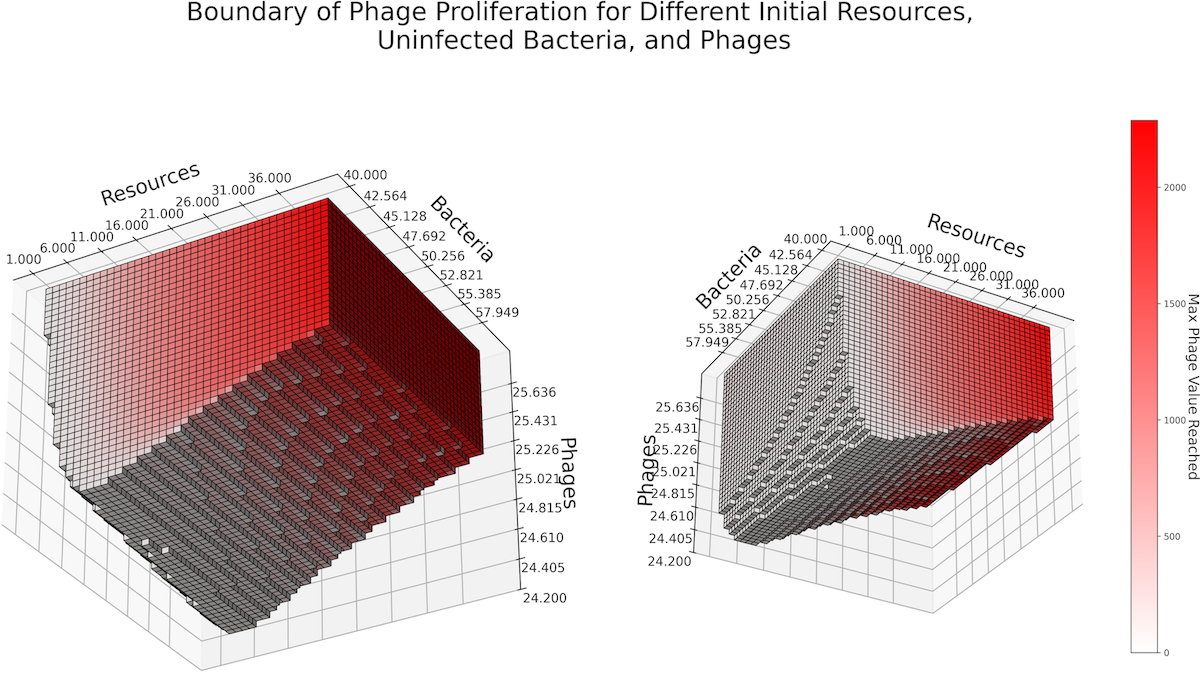
\includegraphics[width=1\textwidth]{Plots/Created/PP/3d_plot_resource_bacteria_phage.png}
    \centering
    \caption{
        A 3D plot of phage proliferation, dependent on the initial resource, uninfected bacteria, and phage population. 
        Color scaling from white to red; the color is dependent on the maximum phage population reached. 
        Zoomed into a small area of interest, zooming out does not offer much more information. 
        In the grand scheme of things, the initial presence of bacteria and resources has little effect on whether phages can proliferate. 
        On a larger initial resource and uninfected bacteria axis range, the boundary becomes essentially flat. 
        \label{fig:created:3D_phase_portrait}
    }
\end{figure}

\section{Plotting Parameter Change – $3\times 2\times 3$ Model}
Now that we have identified the most important parameters in the Golding model, we can analyze how the curve shapes change across a range of parameters for a larger model. 
Understanding how multiple parameters affect the output is crucial. 
As the complexity of the model input increases, interactions and their corresponding parameter values play a crucial role in determining which phage or bacteria can survive. 
The interactions (or lack thereof) will influence the output of the graphs. 

The larger model will exhibit similar but slightly different behavior than a $1\times 1\times 1$ model due to the multiple interactions occurring simultaneously. 
A combination of interactions now explains the population curves. 
The differing parameter values across each interaction will influence how fast each population can grow and decline, which will have cascading effects on the values of other populations. 

A $3\times 2\times 3$ model was chosen because it is situated on the boundary between adding too many phages, bacteria, or resources that would otherwise clutter the plot with lines while still offering behavior that can be compared against one another. 
The $3\times 2\times 3$ graph network used can be found in \Cref{fig:ss:example_network}, with the default parameter values listed in \Cref{tab:appendixE:complex_model}. 
$B_0$ is infected by $P_1$ and $P_2$, and consumes $R_0$ and $R_1$. 
$B_1$ is infected by $P_0$ and $P_2$, while consuming $R_2$. 

\Cref{fig:created:r_beta_washout_0} and \Cref{fig:created:r_beta_washout_0.02} show a $7\times7$ matrix of subfigures between washout rates of 0 and 0.02. 
Each subfigure uses a different combination of $r$ and $\beta$ parameter values. 
The adsorption rate and burst size were chosen because they had the most significant effect on the phage population. 
These results demonstrate that even when controlling the two most important parameters that drive phage growth, secondary, less important parameters and interactions still influence the outcome. 

All initial phage values started at 10. 
This was specifically chosen to illustrate how, although the phage values all start the same, the different parameter values and interactions ultimately influence population growth. 
It was selected to provide context and illustrate how parameter values and interactions ultimately affect the progression of a population. 

If $r$ or $\beta$ is equal to Original, then the simulation uses the original parameter values as defined in \Cref{tab:appendixE:complex_model}, otherwise each $r$ and each $\beta$ parameter interaction has the value listed in the subfigure title. 

The columns and rows of each figure illustrate how a change in parameter value affects the curve while keeping the other parameters constant. 
A visualization of which phages can infect which bacteria and which bacteria can consume which resources can be seen in the $3 \times 2\times 3$ model in \Cref{fig:ss:example_network}. 
$P_0$ infects $B_1$, $P_1$ infects $B_0$, and $P_2$ infects $B_0$ and $B_1$. 
$B_0$ consumes $R_0$ and $R_1$, while $B_1$ consumes $R_2$. 
Washin and washout are included, where washin $\omega^i_r$ is set such that $\omega^i_r = \omega^o \cdot R_r$, where $R_r$ is the initial resource concentration for resource $r$. 

In $r, \beta, \omega^o=\text{Original}, \text{Original}, 0$, the graph shows how the different parameter values for each interaction uniquely affect the growth rate of each entity, especially the phage population ($P_0$=blue, $P_1$=green, and $P_2$=purple). 
All phages start at the same population level of 10. 
$P_2$ has the fastest initial growth rate until $t=4$, at which $P_1$ overtakes $P_2$. 
$P_2$ reaches its peak population count before $P_0$ or $P_1$, but despite the slower initial growth, $P_0$ and $P_1$ eventually overtake $P_2$ in total phage population. 
$P_2$ also reaches its peak before decreasing in population. 
The complete extinction of the bacteria has been delayed long enough that, at trace amounts, phage reduction still occurs despite the bacteria’s continued existence. 
The peak times for $P_0$, $P_1$, and $P_2$ are $t=6.33, 7.99, 4.52$, a difference of $3.47$ time units. 
This illustrates how the other parameter values influence the growth and competition of phages for bacteria, as well as the impact these parameters have on the phage populations. 

Contrast $r, \beta, \omega^o=\text{Original}, \text{Original}, 0$ (the previous paragraph) with the phage population dynamics of $r, \beta, \omega^o = \text{Original}, 100, 0$, the phage populations show less notable dynamics. 
The time of peak values are more similar and consistent with one another ($t=5.50, 7.01, 6.78$, a maximum difference of 1.51-time units). 
By decreasing the variability of the $\beta$ values, the system’s dynamics have undergone significant changes. 
Sobol suggested that changing $\beta$ will not have a large effect on the time of peak values, but when combined with other interactions, the parameter effect can propagate through the network. 

The phage population curve all appears the same, with slightly slower growth rates compared to $r, \beta, \omega^o=\text{Original}, \text{Original}, 0$. 
There is no crossing of phage population count, unlike with $r, \beta, \omega^o=\text{Original}, \text{Original}, 0$. 
The crossing of phage populations highlights how one phage population performs better than the other, especially when compared to different situations where the cross does not occur. 

As the washout term changes, the choice of parameters becomes more critical. 
The top row of \Cref{fig:created:r_beta_washout_0.02} $(\omega^o = 0.02)$ shows how the phages and resources died out relative to the top row of \Cref{fig:created:r_beta_washout_0} $(\omega^o = 0)$. 
Even with a high burst value, the phages were unable to overcome the pressure from the washout. 
The phages were not able to proliferate under these conditions. 

However, by changing the $r$ value from $r=0.001$ to $r=0.009$, with $\beta \geq 21.6$, the phages were able to proliferate at a higher washout rate. 
Small changes in parameter values can have a drastic impact on outcomes.

The highlighted examples demonstrated the dynamics and influence that multiple agents can have on the final output. 
These graphs still show some realistic growth curves that can be directly compared against \Cref{fig:created:a_good_curve_linear}. 
However, with the addition of more interactions, phage and bacterial growth differ, where some phages and bacteria die out faster than others. 

\begin{figure}[]
    \centering
    \begin{subfigure}{0.49\linewidth}
        \centering
        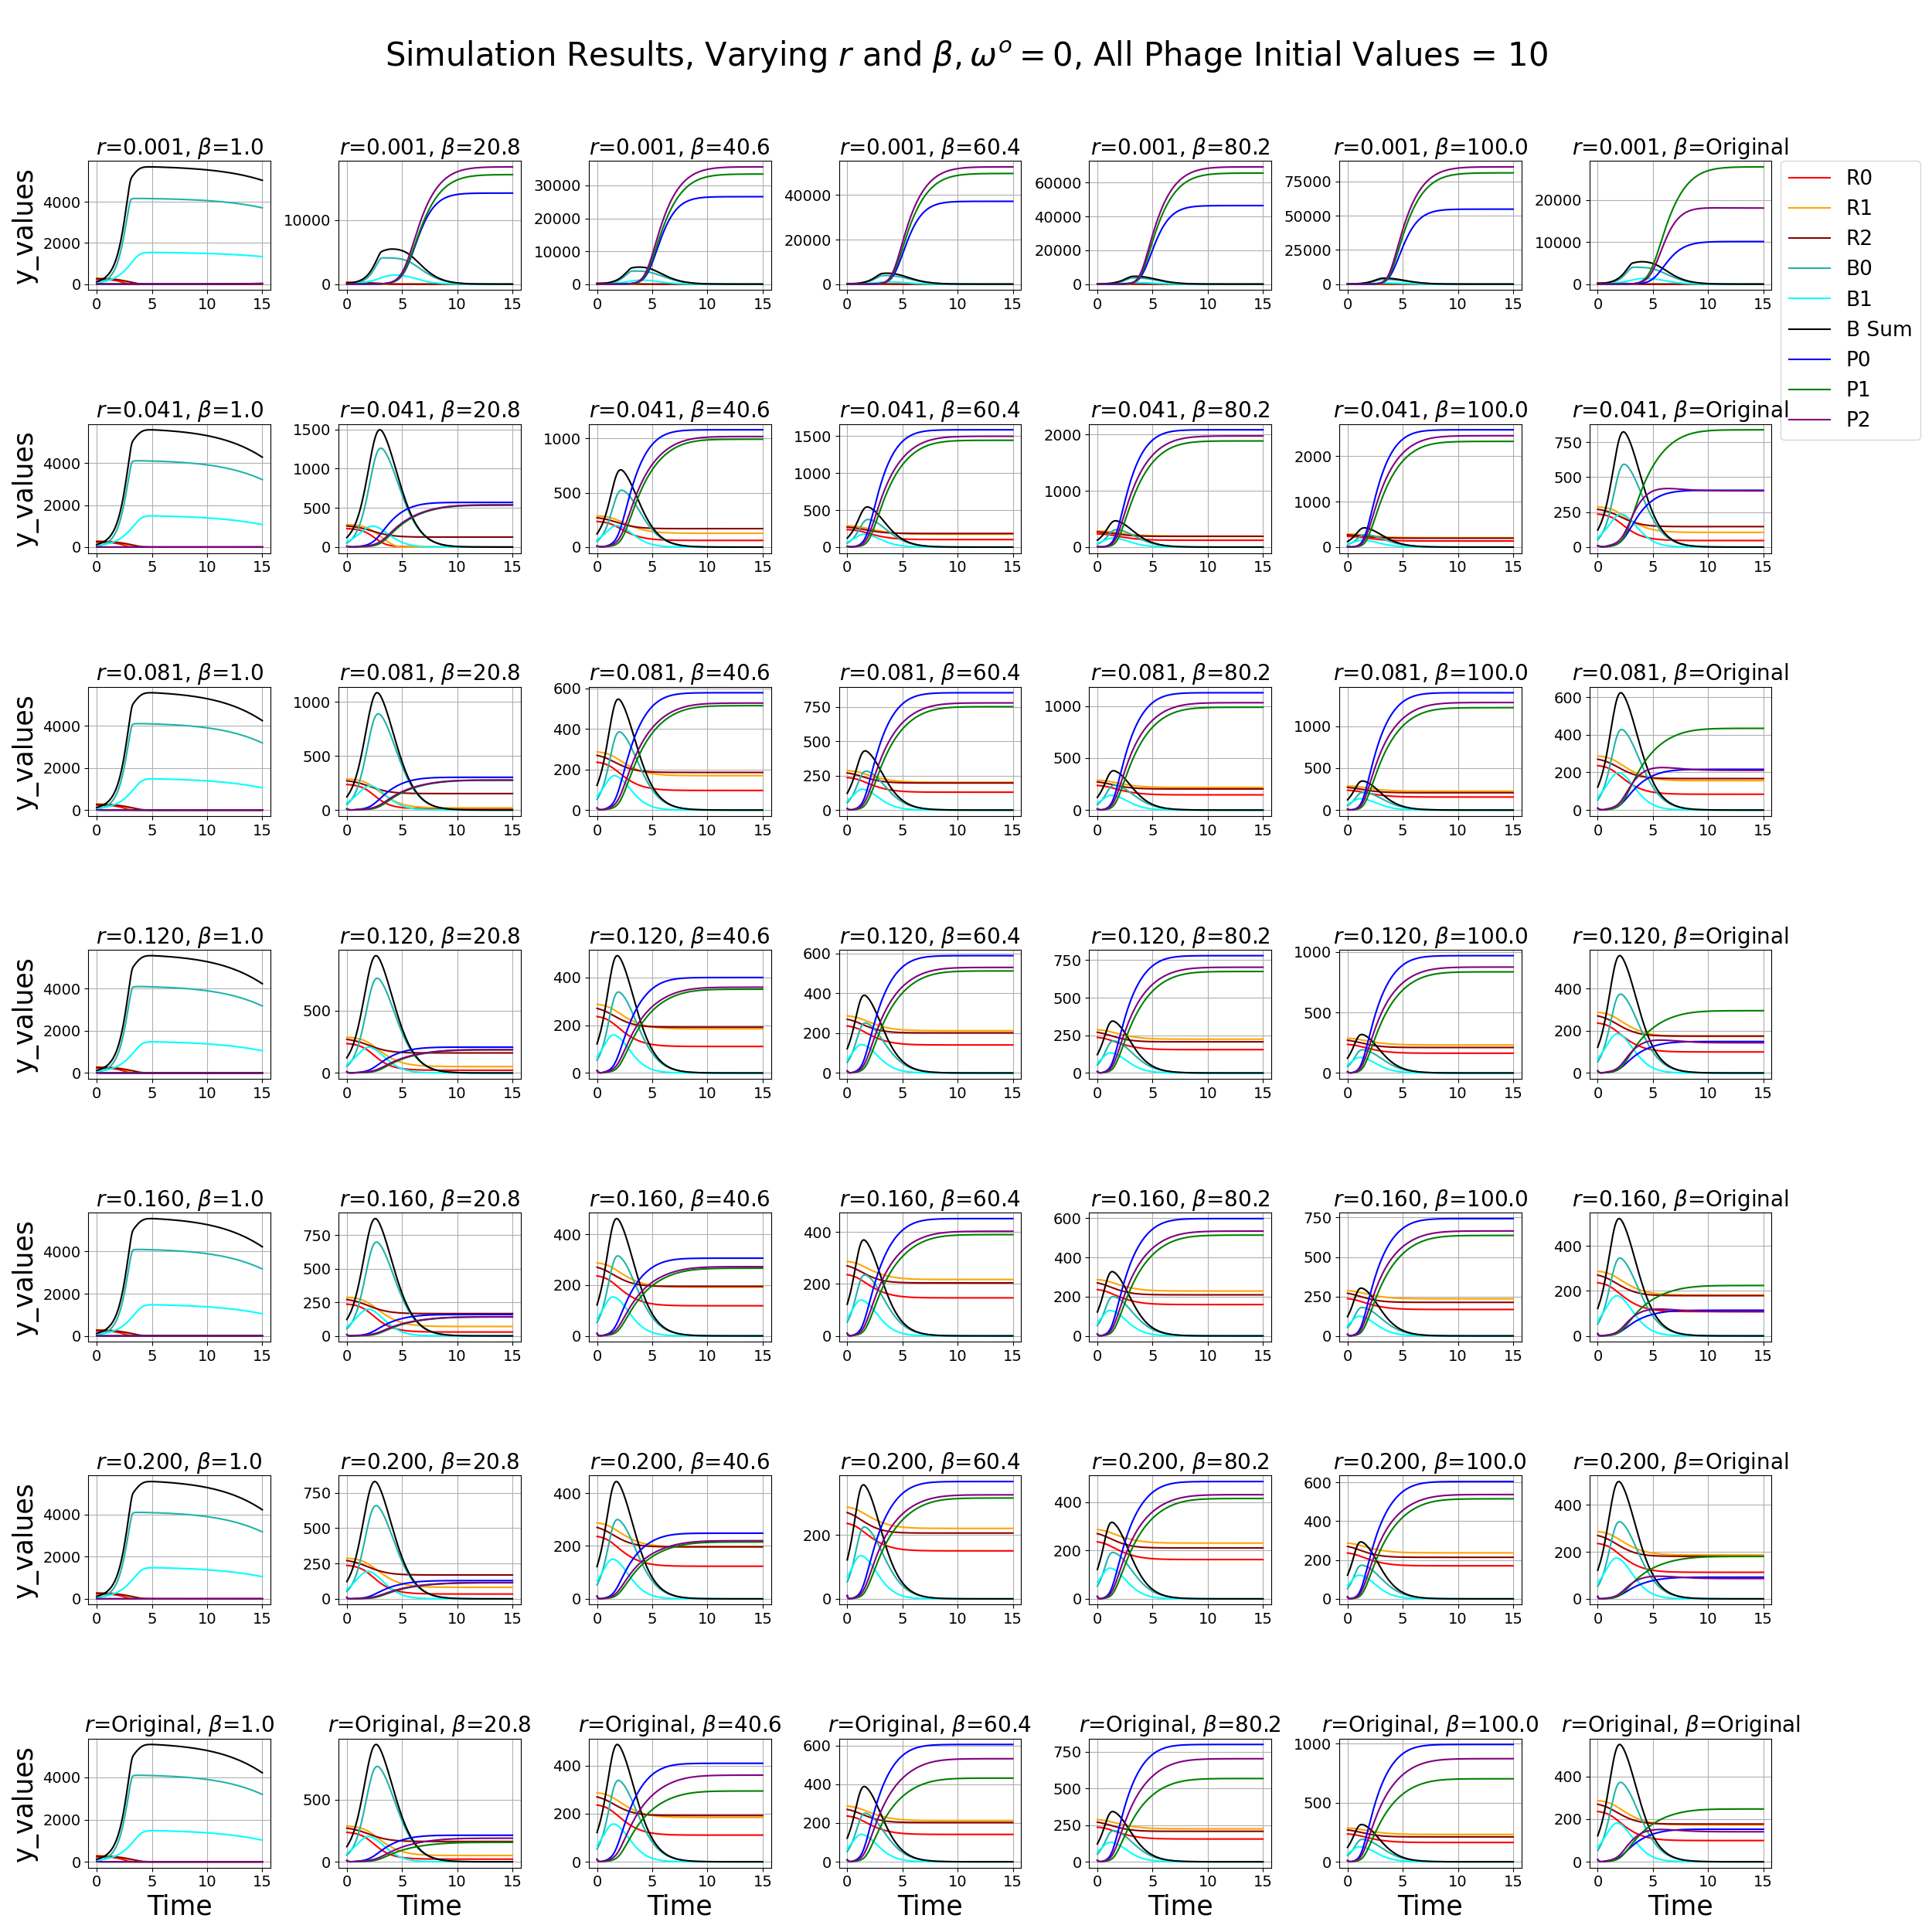
\includegraphics[width=\linewidth]{Plots/Created/UA/r_beta_washout_0.png}
        \caption{
            Washout $\omega^o=0$. 
        }
        \label{fig:created:r_beta_washout_0}
    \end{subfigure}
    \hfill
    \begin{subfigure}{0.49\linewidth}
        \centering
        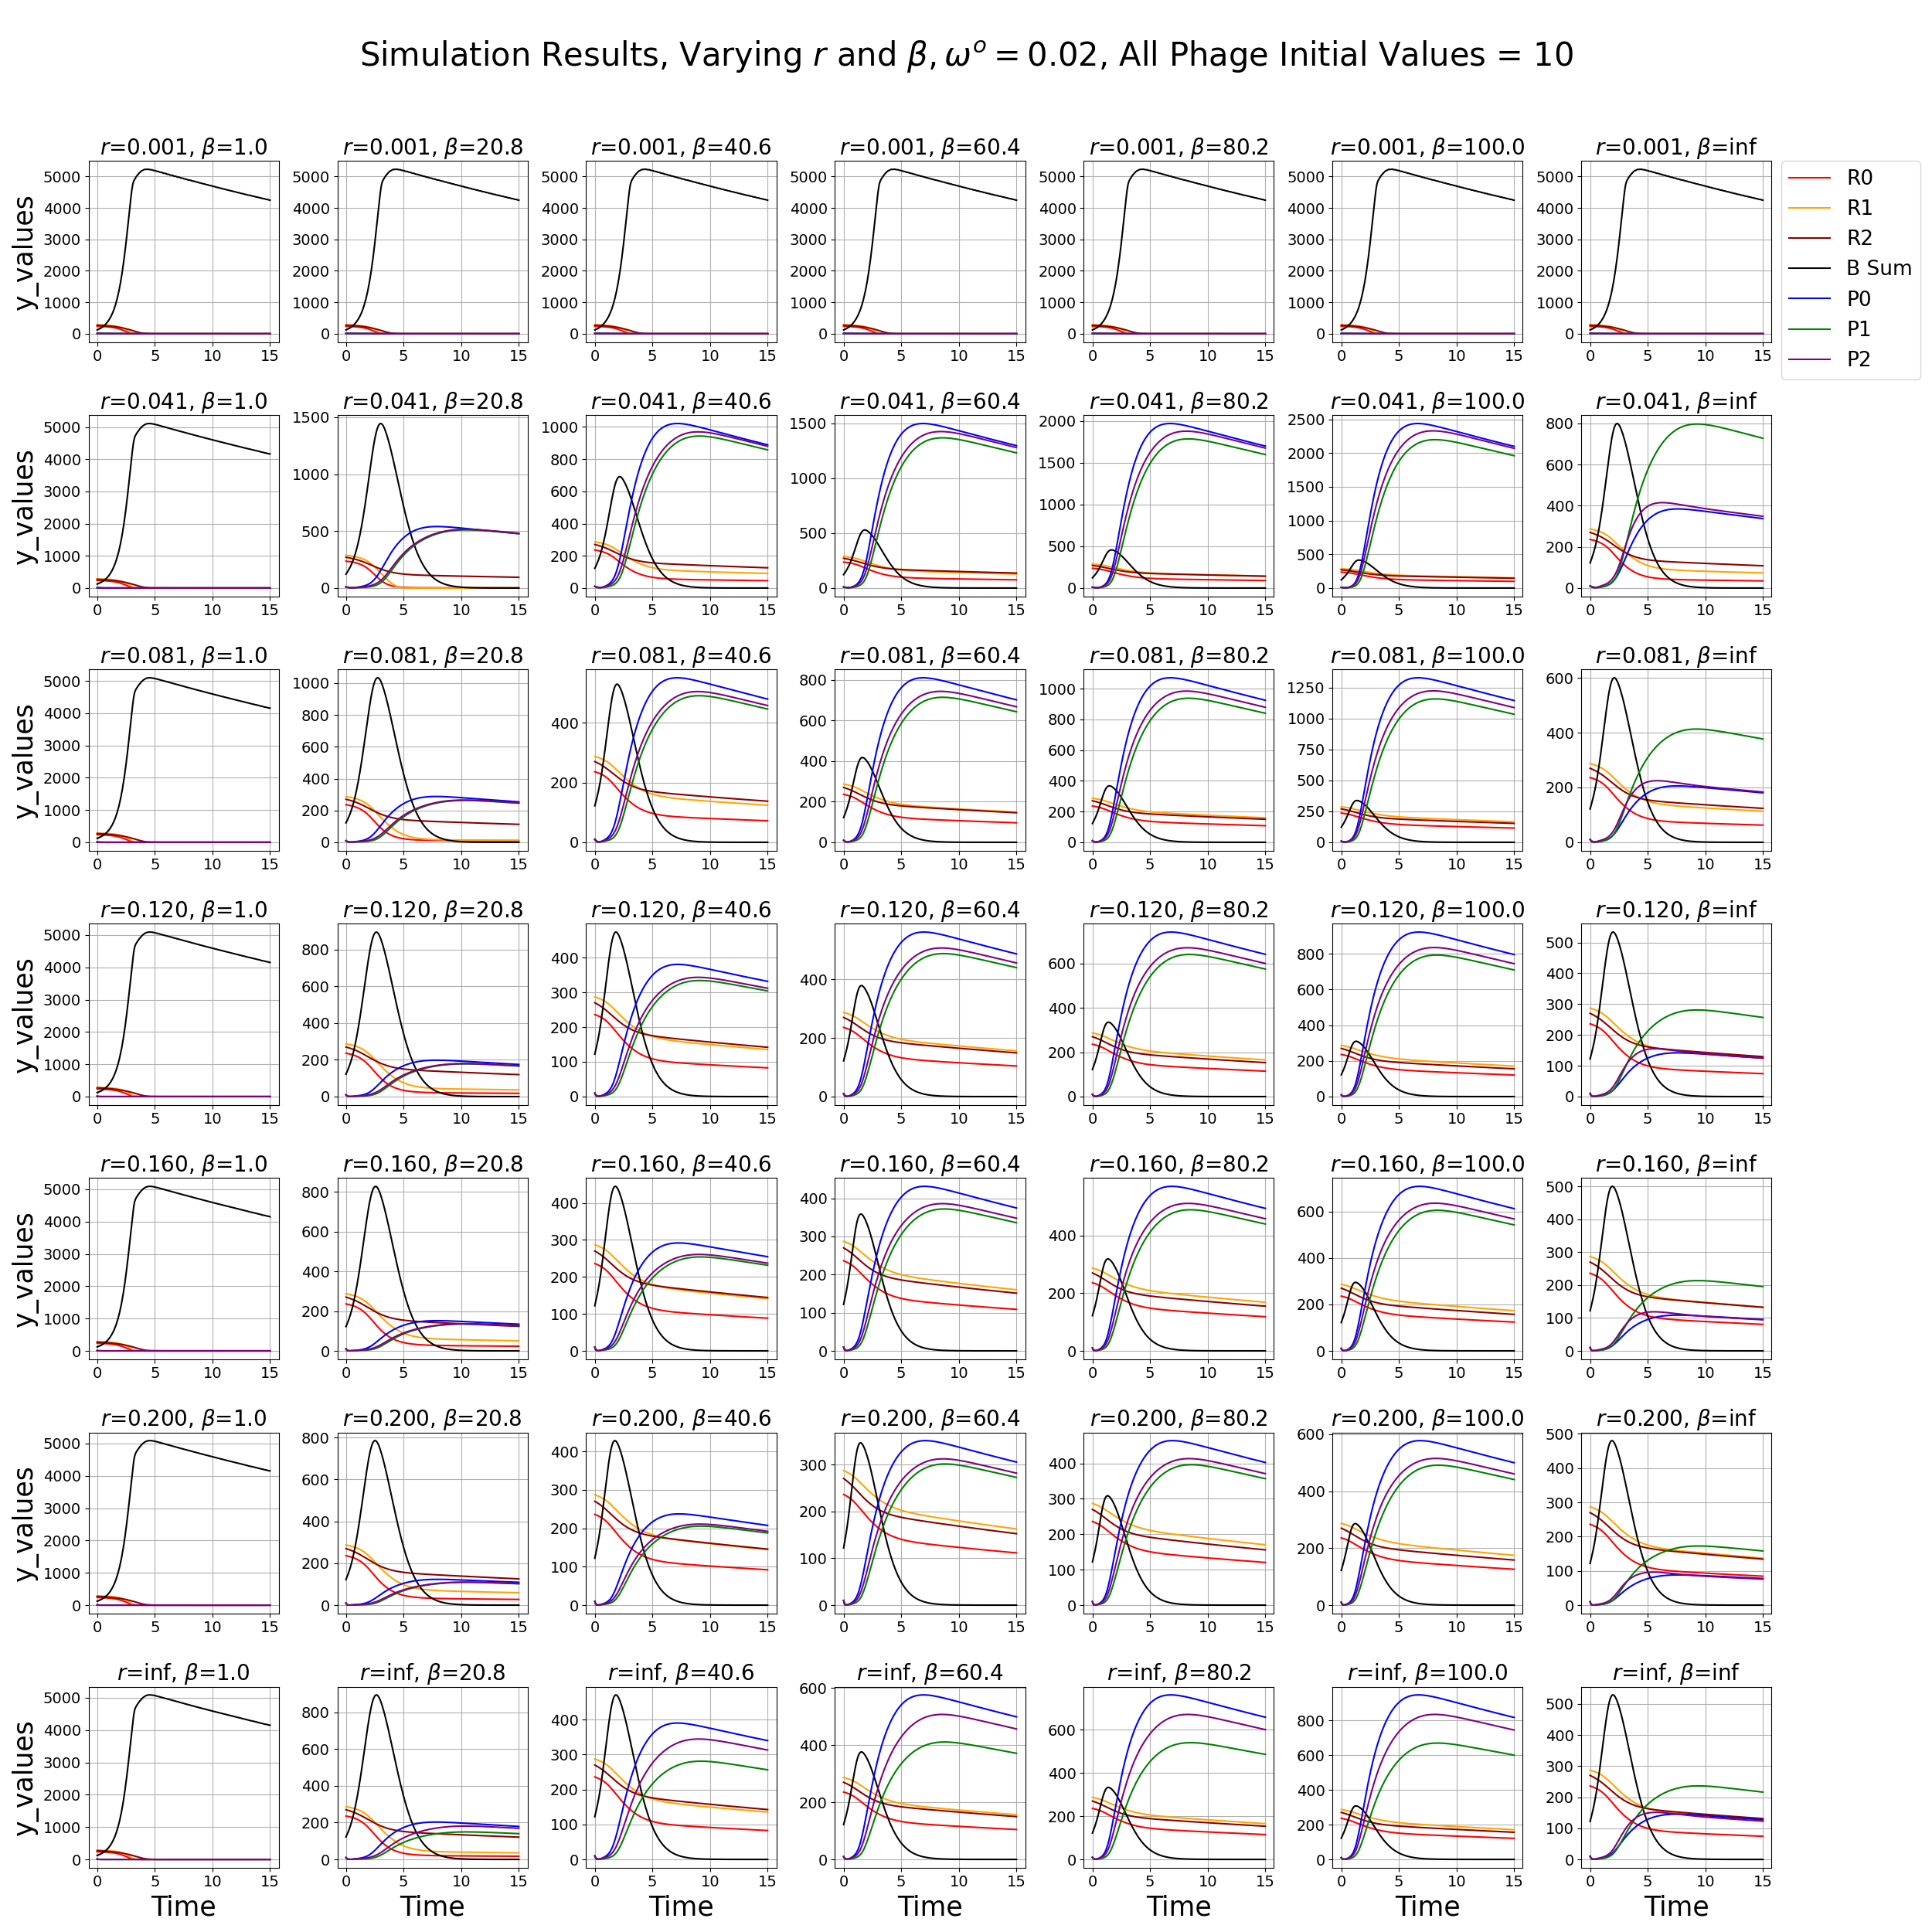
\includegraphics[width=\linewidth]{Plots/Created/UA/r_beta_washout_0.02.png}
        \caption{
            Washout $\omega^o=0.02$. 
        }
        \label{fig:created:r_beta_washout_0.02}
    \end{subfigure}
    \caption{
        Varying adsorption rate $r$, $\beta$, $\omega^o$ and $\omega^i$. 
        The default values for the parameters can be found in \Cref{tab:appendixE:complex_model}. 
        All initial phage population values were set to 10. 
        Washout values are set such that $\omega^i_r = \omega^o \cdot R_r$. 
    }
\end{figure}

\section{Phage and Bacteria Survivability Analysis For A $20\times20\times10$ System}
In the context of large communities, it is essential to understand how different conditions will influence whether a phage or bacterial population will survive. 
Different interactions and environmental factors will influence the community’s evolution. 
Sometimes, populations of phages or bacteria will die out due to external factors, such as a lack of resources or bacteria to consume or infect, natural degradation, or exposure to external factors like UV light. 

Using the simulation framework, I created and analyzed a $20\times20\times10$ system using the adapted Golding model. 
I selected two parameters, $\tau$ and $\beta$, to run a survivability analysis using the adapted Golding model. 

A phage is considered to have survived if its final population exceeds 1 at the end of the simulation. 
A bacterial population likewise is considered to have survived if the final population of uninfected bacteria is greater than 1. 
Washout removes phages and bacteria from the system over time unless a delicate balance of coexistence is maintained. 
Washin provides a continuous supply of new resources to support bacterial growth, which in turn supports phage infection. 
Meanwhile, washout prevents the phage population from growing too large and infecting all bacteria.

Each phage is guaranteed to interact with at least one bacterium but no more than two bacteria. 
Each bacterium interacts with at least one phage and one resource but not more than two phages and two resources. 
Every resource interacts with at least one bacterium and, at most, three bacteria. 
The parameter values were randomly selected from a uniform distribution within the Sobol analysis value ranges (\Cref{tab:appendixE:Sobol_analysis_values}). 
\Cref{fig:ss:example_large_network} shows the network interactions. 

\Cref{fig:created:survivability} shows the phage and bacteria survivability matrix. 
It appears that there is an inverse relationship between phage and bacterial survivability. 
If the phages survived, the bacteria died out. 
If the bacteria survived, the phages did not survive. 
The phages only died out with small burst sizes, $\beta$, while otherwise would consistently survive. The small burst size ensured that the phages could not proliferate in time. 
Once the burst size became large enough, around $\beta = 3$, more than half of the phages were able to survive. 
The bacteria only survived with small burst sizes $\beta$. 
For large burst sizes, the phages would grow too fast and infect the bacteria. 

$\tau$ had less of an influence in survivability than $\beta$ did, except for when the $\beta$ values were less than 20. 
As $\tau$ increases, fewer phages survive, and more bacteria survive. 
$\tau$ determines how fast a bacterium goes through the infection process, so as $\tau$ increases, fewer phages will survive. 
The bacterium takes longer for the infection process to complete, so there is a greater chance for the phages and infected bacteria to be washed out before more phages can be created. 

For the most part, the competitive exclusion principle is respected. 
The majority of the simulations resulted in less than 10 uninfected bacteria surviving. 
For small burst sizes, there were more than 10 surviving bacteria. 
However, this is a consequence of the limited simulation length. 
I expect more bacterial populations to die out as the simulation length increases.

\begin{figure}[]
    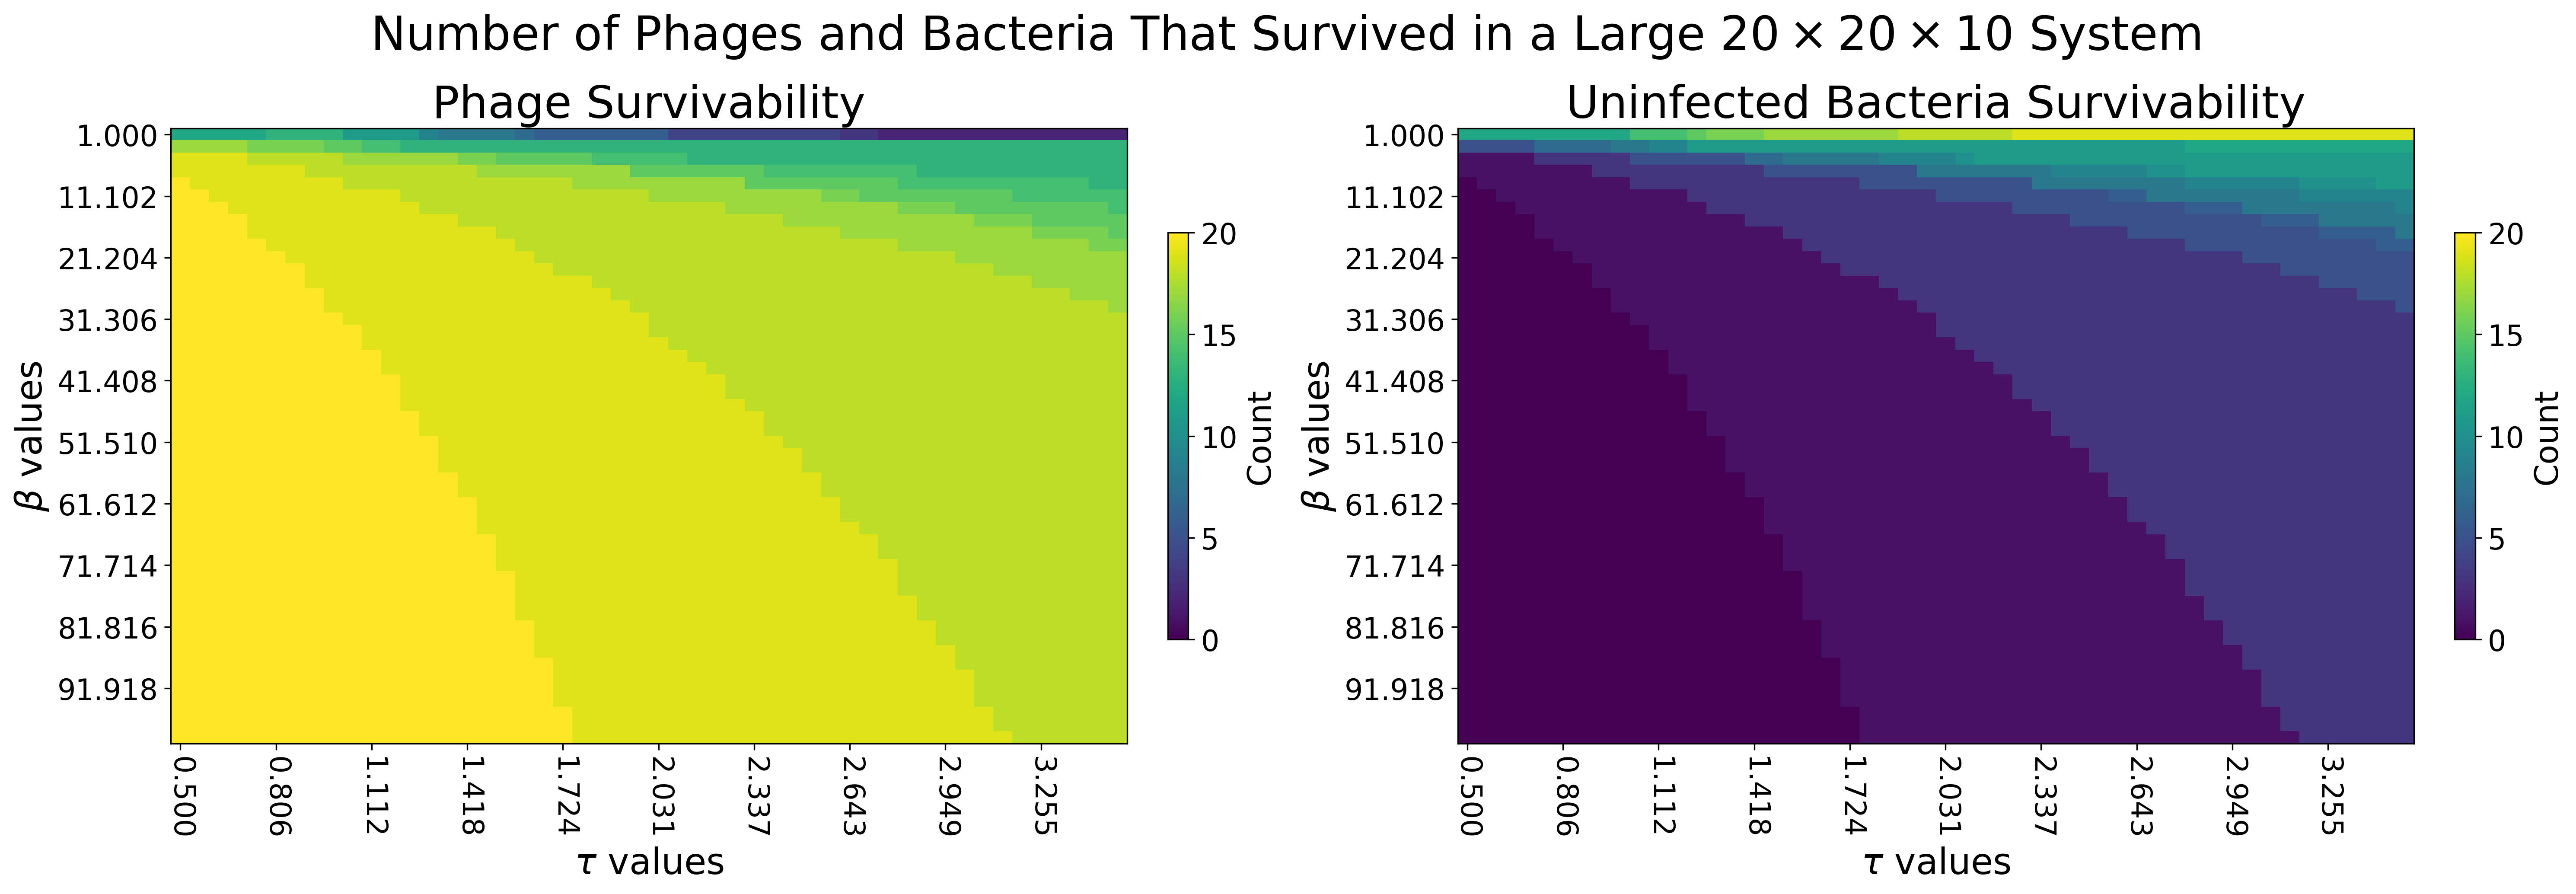
\includegraphics[width=1\textwidth]{Plots/Created/phage_bacteria_survivability.png}
    \centering
    \caption{
        The survivability matrix for phages and bacteria by changing $\tau$ and $\beta$ in a $20\times 20\times 10$ network. 
        The output graph for the default parameter values for an extensive $20\times 20 \times 10$ network. 
        Parameter values were randomly chosen in the interval given by \Cref{tab:appendixE:Sobol_analysis_values}. 
    }
    \label{fig:created:survivability}
\end{figure}

\subsection{Debris Term}
\label{sec:results:debris}
A recently published paper \citet{deyEmergentHigherorderInteractions2025} utilizes the Golding model, incorporating a new term: debris. While running their simulations and experiments, the model’s results would diverge from their experimental work. 
They hypothesized that freshly lysed bacteria still have biomarkers that phages can detect and attach to. 
Incorporating the debris term, which acts as an additional death term for phages, improved the model’s alignment with the experimental data.
The debris term can also encompass bacterial phage defenses (\Cref{sec:literaturereview:bacterial_defense_against_phages}). 
The ODE equation from the generalized Golding model that describes the phage behavior can be rewritten as: 
\[
    \frac{dP_p}{dt} = \sum_{b\in B}\beta_{p b}\cdot\frac{M}{\tau_b} \cdot I_{b_M} - r_{p b}\cdot(U_b + \sum_{k=1}^{M} I_{b_k})\cdot P_p - w^o \cdot P_p \mathcolor{red}{- d_{pb} \cdot P_p}
\]
\Cref{fig:created:debris_model} shows how debris $d$ affected the growth curves of the phages and bacteria in comparison to no debris term, \Cref{fig:created:no_debris_model}. 
Without the debris term, only one uninfected bacteria survived, and every phage survived except for one phage that died due to the washout. 
Three uninfected bacteria species reached more than 1,000 uninfected bacteria at any point in the simulation time, and only two infected bacteria species reached more than 1,000 infected. 
The maximum total bacterial population reached was 6,620 bacteria. 

With the debris term included, different results are apparent. 
Three uninfected bacteria survived, and four different uninfected bacteria strains ever reached a population value of greater than 1,000 at any point in time during the simulation. 
Only one bacteria strain ever reached more than 1,000 infected bacteria, 
The ending bacteria value is 12,000, almost double the maximum bacteria population reached without debris. 
On average, there were significantly fewer phages at the end of the simulation than in the control without debris. 
No phage population exceeded 2,000 with debris, whereas two phage populations reached more than 2,000 phages without debris. 

The debris term more accurately models real communities as phages can randomly deactivate, for example, by UV radiation or phage defense mechanisms. 

\begin{figure}
    \centering
    \begin{subfigure}{1\linewidth}
        \centering
        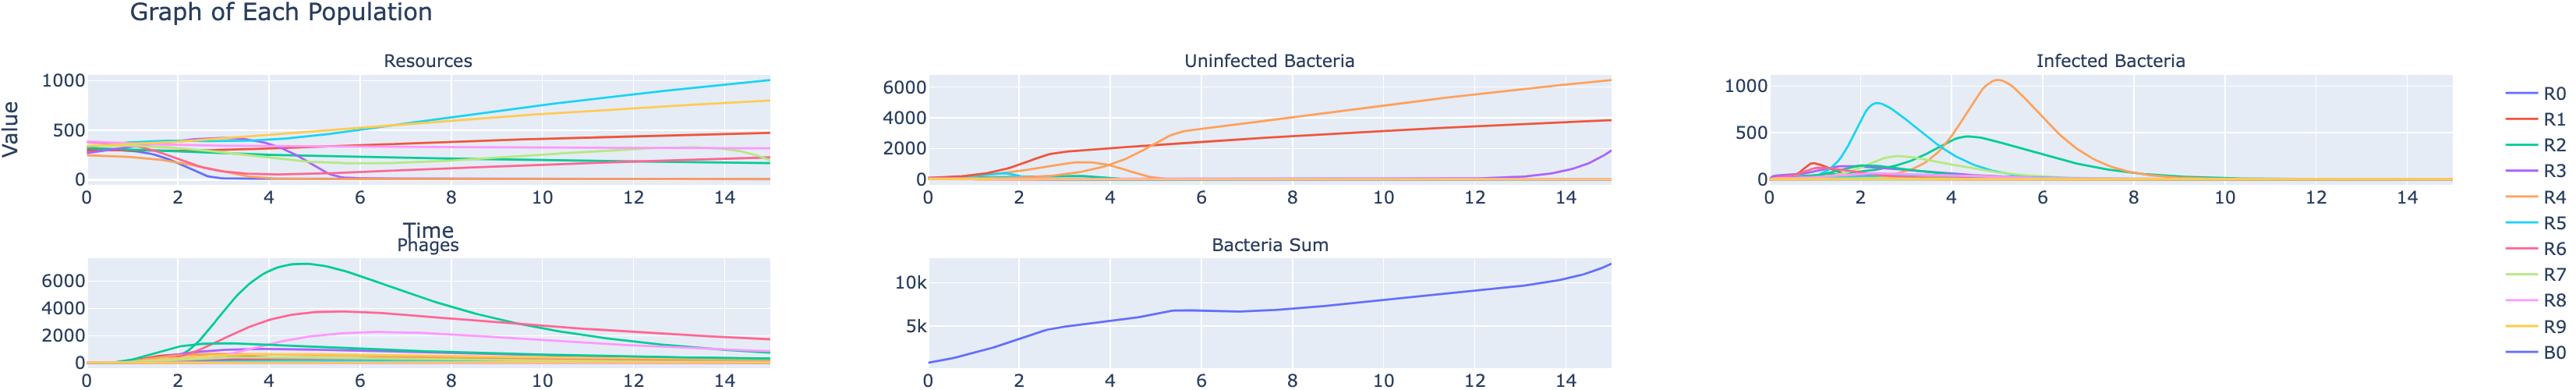
\includegraphics[width=\linewidth]{Plots/Created/debris.png}
        \caption{
            The $20\times20\times10$ model with a debris factor included. 
        }
        \label{fig:created:debris_model}
    \end{subfigure}
    \hfill
    \begin{subfigure}{1\linewidth}
        \centering
        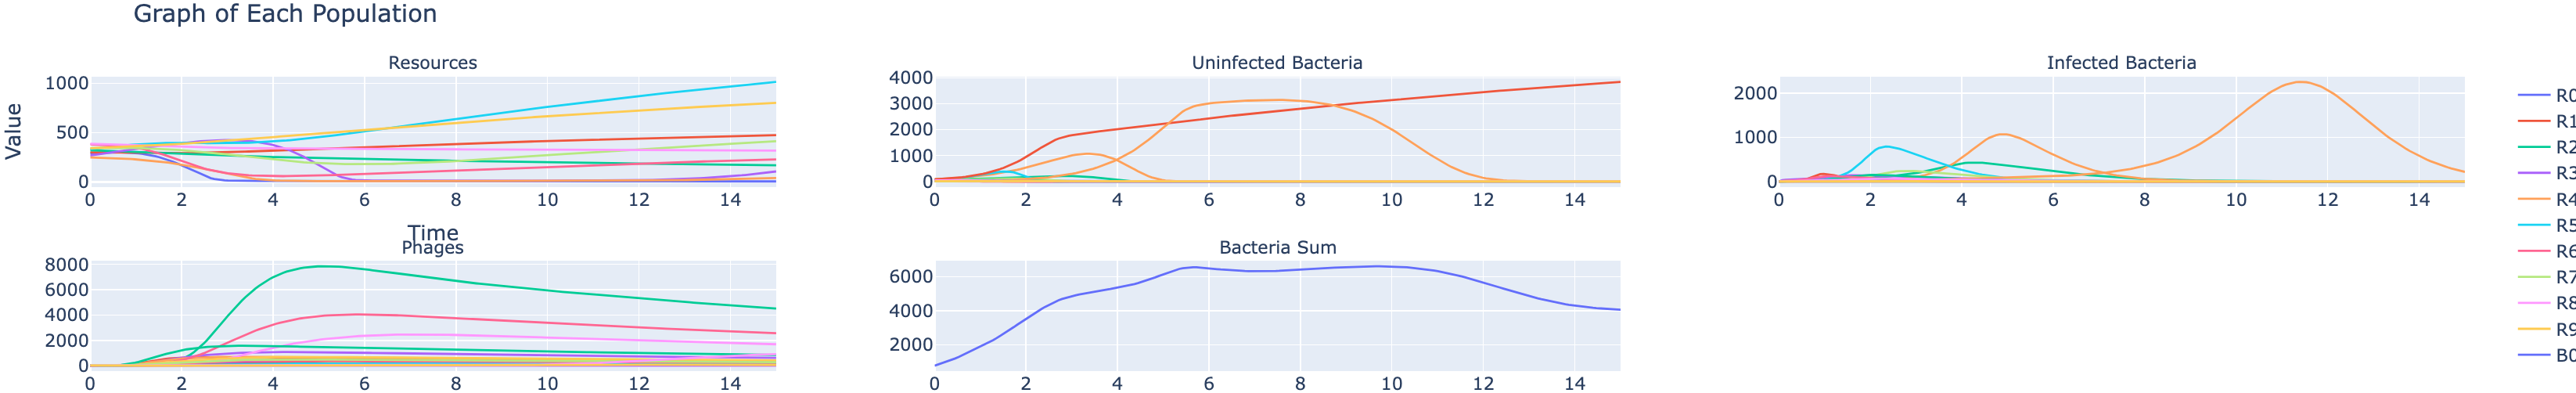
\includegraphics[width=\linewidth]{Plots/Created/no_debris.png}
        \caption{
            The $20\times20\times10$ model without the debris factor included. 
        }
        \label{fig:created:no_debris_model}
    \end{subfigure}
    \caption{
        A large $20\times20\times10$ model with a debris parameter added. 
        The debris parameter values were randomly and uniformly selected between 0.01 and 0.2 for each phage-bacteria interaction. 
        Washin of resources and washout is included. 
    }
    \label{fig:created:debris}
\end{figure}